\documentclass[preprint]{elsarticle}

\usepackage{fixme}
\usepackage{amsmath,amssymb}
\usepackage{xcolor}
\usepackage{graphicx}
\usepackage{xspace}
\usepackage{booktabs}
\usepackage{dsfont}
\usepackage{tabularx}
\usepackage{stmaryrd}
\usepackage{tikz}
\usetikzlibrary{arrows,arrows.meta,automata,positioning}
\usepackage{mathrsfs}
% \usepackage{hyperref}
\usepackage{amsthm}
% Theorem environments
\newtheorem{theorem}{Theorem}[section]
\newtheorem{lemma}[theorem]{Lemma}
\newtheorem{corollary}[theorem]{Corollary}
\newtheorem{proposition}[theorem]{Proposition}
\newtheorem{claim}[theorem]{Claim}
\newtheorem{fact}[theorem]{Fact}
\newtheorem{question}[theorem]{Question}

% Definition-like environments
\theoremstyle{definition}
\newtheorem{definition}[theorem]{Definition}
\newtheorem{notation}[theorem]{Notation}

% Remark-like environments
\theoremstyle{remark}
\newtheorem{remark}[theorem]{Remark}
\newtheorem{example}[theorem]{Example}

\biboptions{longnamesfirst,semicolon}
\usepackage[
    colorlinks=true,
    linkcolor=blue,
    citecolor=green!50!black,
    urlcolor=red!70!black,
    filecolor=magenta
]{hyperref}
\newcommand{\model}{\M}
\newcommand{\prop}{\mathsf{Prop}}
\def\M{\mathcal{M}}

\renewcommand{\iff}{\text{\it iff}}

\newcommand{\form}{\mathsf{Form}}

\newcommand{\modsabx}[2]{{#1}^x_{-#2}}
\newcommand{\modsab}[3]{{#1}^{#3}_{-#2}}
\newcommand{\modswapx}[2]{{#1}^x_{*#2}}
\newcommand{\modswap}[3]{{#1}^{#3}_{*#2}}
\newcommand{\modbridx}[2]{{#1}^x_{+#2}}
\newcommand{\modbrid}[3]{{#1}^{#3}_{+#2}}

\newcommand{\sabbisim}{\leftrightarroweq^-}
\newcommand{\swapbisim}{\leftrightarroweq^{\shortleftarrow}}
\newcommand{\bridbisim}{\leftrightarroweq^{+}}
\newcommand{\truthset}[3]{\llbracket{#1}\rrbracket_{#2}^{#3}}

\newcommand{\tup}[1]{\langle{#1}\rangle}

\DeclareMathOperator{\dsab}{\tup{\mathsf{sb}}}
\DeclareMathOperator{\dbr}{\tup{\mathsf{br}}}
\DeclareMathOperator{\dsw}{\tup{\mathsf{sw}}}

\begin{document}

\begin{frontmatter}

% \title{Bisimulations for Probabilistic \\ Relation-Changing Modal Logics}
\title{Tilting the Odds: Relation-Changing Modal Logics for Probabilistic Systems}
\author[unc,conicet]{Raul Fervari}
\author[aveiro,coimbra]{Daniel Figueiredo}
\author[aveiro]{Manuel A. Martins}
\author[unc]{Gonzalo Zigar\'an}

\address[unc]{
    FAMAF, Universidad Nacional de C\'ordoba, Argentina
}

\address[conicet]{
    Consejo Nacional de Investigaciones Cient\'ificas y T\'ecnicas, Argentina
}

\address[aveiro]{
    Center for Research and Development in Mathematics and Applications (CIDMA), Universidade de Aveiro, Portugal
}

\address[coimbra]{
    Association for Innovation and Biomedical Research on Light and Image, Portugal
 }

\begin{abstract} 
Relation-changing logics are formalisms for describing dynamic phenomena over discrete models. Two main approaches have been proposed to reason in this setting: syntactic ones, where the model is changed by logical operators in the language, and semantic ones, where the change in the system is parameterized by the model itself. In recent years, the relation-changing paradigm has been extended in several directions, for instance to paraconsistent and fuzzy settings. In this work, we introduce relation-changing logics over probabilistic transition systems. Specifically, we propose three operators: a local sabotage modality, which reduces the probabilities of the edges adjacent to the evaluation point; a local bridge modality, which instead increases them; and a local swap modality, which reverses the probability between two adjacent nodes. We study the semantic effects of adding these modalities. In particular, we investigate novel notions of probabilistic bisimulation and establish their adequacy through the corresponding invariance and Hennessy-Milner results.
\end{abstract}

\begin{keyword}
Relation-Changing \sep
Probabilistic Logics \sep
% Probabilistic Kripke Model \sep
Bisimulation \sep
Sabotage Logic \sep
Bridge Logic \sep 
Swap Logic
\end{keyword}

\end{frontmatter}

\section{Introduction}

Probabilistic transition systems can be represented by different kinds of models. Markov chains, for example, are a familiar model in this setting, while probabilistic automata provide a broader framework (see, e.g.,~\cite{Segala95}). Logical languages can then be used to describe system properties and reason about system behavior. These include temporal logics, used in PRISM to specify properties of Markov chains~\cite{Kwiatkowska2007} and to reason about knowledge~\cite{HT93}. Finally, Probabilistic Modal Logics are specifically tailored to  reasoning about probabilistic Kripke structures (see, e.g.,~\cite{ALDINI2024109167}) and provide a more general view on transition systems.

Relation-changing formalisms provide another perspective on transition systems. They are discrete-state models in which the accessibility relation can change in response to an event, such as traversing an edge. These changes can be semantically encoded in the model or introduced syntactically through operators in the language. In switch graphs, for example, changes to the relation are encoded in the model structure itself~\cite{GabbayM12}. Classical modal logic can be used to explore such a model without itself changing the relation. Instead, the prescribed updates occur when designated edges are traversed. Alternatively, one can start with a standard Kripke structure and use a logic whose syntax includes relation-changing operators. Sabotage and bridge logics, for example, include operators that modify the model during formula evaluation, so that the remaining subformula is evaluated on the modified model~\cite{ArecesFH15,Aucher&vanBenthem&Grossi18,Fervari14}.
This kind of dynamic behavior can be also found in many applications of logics interpreted over graph-like structures, such as logics of public announcements and its relatives in epistemic logic (see, e.g.,~\cite{Plaza89:lopc,FervariV19}), logics for resource allocation such as separation logics (see, e.g.,~\cite{OHearn19,DemriD15})  and epistemic planning~\cite{BolanderA11}, to name a few.
% \textcolor{red}{Should we mention logics with public announcements?}

In recent years, the relation-changing paradigm has been extended to several classes of models, including paraconsistent~\cite{CostaFM23}, weighted~\cite{FRMC19}, fuzzy~\cite{FFM25}, and labeled models~\cite{CFMS25,FMB18}. Applications and computational tools have also emerged. For instance, \cite{FRMC19} presents a tool for a probabilistic setting based on a particular choice of weights. In \cite{MFAPCB24}, a related approach is applied in a practical setting, illustrating its potential for real-world applications. Other case studies include~\cite{FB18,SMF21}.

This work advances this line of research by introducing relation-changing operators for probabilistic systems, rather than restricting attention to predefined models with limited expressive power. Although relation-changing approaches have also been studied in fuzzy settings~\cite{FFM25}, the probabilistic setting is not simply a special case of the fuzzy one. In particular, the outgoing transition probabilities at each state must sum to one, so changing one transition may require corresponding adjustments to others. This normalization constraint also poses new challenges for the metatheoretic analysis of the resulting logics. 

In this article we present a probabilistic setting for relation-changing logics, and study associated probabilistic bisimulation notions. We expand the results presented in~\cite{FFM25b}, by providing full proofs, more detailed discussions, examples of use, and incoporating new results. In particular, one of the novel contributions herein with respect to~\cite{FFM25b} is the proof of Hennessy-Milner results for the operators we studied.

\paragraph{Outline} In Section~\ref{sec:pml} we introduce the syntax, semantics and bisimulation notion for the basic probabilistic modal logic that we consider the basis of our framework. Section~\ref{sec:prcml} is devoted to exploring probabilistic versions of sabotage and bridge modalities. Then, in Section~\ref{sec:bisimulation}, we present their associated notions of bisimulations and show their corresponding invariance theorems. Therein, we also investigate respective Hennessy-Milner classes and prove their adequacy. We conclude in Section~\ref{sec:final} with some remarks and future lines of work.
\section{Probabilistic Modal Logic}
\label{sec:pml}

\subsection{Syntax and Semantics}

In this section we present some preliminary notions over probabilistic logics. 
In what follows, let $\prop$ be a non-empty countable set of atomic propositions. Also, for every relation $E\subseteq S\times S$, we use the abbreviation:
\[ 
    E[U]=\{v \in S  \mid (u,v)\in E \text{ for some }u\in U \}. 
\] 

\begin{definition} A \emph{probabilistic Kripke model} is a tuple $\M=(W,P, V)$ where:

\begin{itemize}
    \item $W$ is a countable set of states or worlds; 
    \item $P : W \times W \rightarrow [0,1]$ is the transition probability matrix where for all $w \in W$, $\displaystyle\sum_{w' \in W} P(w, w') = 1$;
    \item $V : \prop \rightarrow 2^W$ is a function that assigns to each $p \in \prop$ the set of states in which $p$ holds.
\end{itemize}
\end{definition}

%An execution of PTS \( D = (S,  P, L) \) is represented by a path. Formally, a path \( \omega \) is a non-empty sequence of states \( s_0 s_1 s_2 \dots \) in $S$ where\( P(s_i, s_{i+1}) > 0 \) for all \( i \geq 0 \).


%%% comented text %%%%%
%A path can be either finite or infinite. We denote by \( \omega(i) \) the \( i \)-th state of a path \( \omega \), \( |\omega| \) the length of \( \omega \) (number of transitions), and for a finite path \( \omega_{\text{fin}} \), the last state by \( \text{last}(\omega_{\text{fin}}) \). We say that a finite path \( \omega_{\text{fin}} \) of length \( n \) is a prefix of the infinite path \( \omega \) if \( \omega_{\text{fin}}(i) = \omega(i) \) for \( 0 \leq i \leq n \). The sets of all infinite and finite paths of \( D \) starting in state \( s \) are denoted \( \text{Path}_D(s) \) and \( \text{Path}_D^{\text{fin}}(s) \), respectively. Unless stated explicitly, we always deal with infinite paths.

%In order to reason about the probabilistic behaviour of the DTMC, we need to determine the probability that certain paths are taken. This is achieved by defining, for each state \( s \in S \), a probability measure \( \text{Pr}_s \) over the set of infinite paths \( \text{Path}_D(s) \).\\
%(We should put references how to define such probability measure)

%Below, we give an outline of this construction. For further details, see [41]. The probability measure is induced by the transition probability matrix \( P \) as follows. For any finite path \( \omega_{\text{fin}} \in \text{Path}_D^{\text{fin}}(s) \), we define the probability \( \text{P}_s(\omega_{\text{fin}}) \):
%$$ \text{P}_s(\omega_{\text{fin}}) \triangleq 
%\begin{cases} 
%1 & \text{if } n = 0, \\
%P(\omega(0), \omega(1)) \cdot \dots \cdot P(\omega(n-1), \omega(n)) & \text{otherwise},
%\end{cases}
%$$
%where \( n = |\omega_{\text{fin}}| \). Next, we define the cylinder set \( C(\omega_{\text{fin}}) \subseteq \text{Path}_D(s) \) as:
%$$
%C(\omega_{\text{fin}}) \triangleq \{ \omega \in \text{Path}_D(s) \mid \omega_{\text{fin}} \text{ is a prefix of } \omega \}.
%$$


%\subsection{Probabilistic Computation Tree Logic (PCTL)}

%Specifications for DTMC models can be written in PCTL (Probabilistic Computation Tree Logic)~\cite{baier2008}, a probabilistic extension of the temporal logic CTL (put a reference for it).

%\begin{definition}[\cite{Kwiatkowska2007}] The grammar of PCTL is the  following

%\[
%\Phi ::= \textbf{true} \mid a \mid \neg \Phi \mid \Phi \land \Phi \mid \mathbb{P}_{\sim p}[\phi]
%\]
%\[
%\phi ::= \textsf{X} \, \Phi \mid \Phi \, \mathsf{U}^{\leq k} \Phi
%\]

%\noindent\textit{where $a$ is an atomic proposition, $\sim \in \{<, \leq, \geq, >\}$, $p \in [0,1]$ and $k \in \mathbb{N} \cup \{\infty\}$.}
%\end{definition}




%\begin{definition} Let \( \M = (S, P, L) \) be PTS. For any state \( s \in S \), the satisfaction relation \( \models \) is defined by:
%\begin{itemize}
%\item$
%\M,s \models \text{true} \quad \text{for all } s \in S
%$\item $
%\M,s \models a \iff a \in L(s)
%$\item $
%\M,s \models \neg \Phi \iff s \not\models \Phi
%$\item $
%\M,s \models \Phi \land \Psi \iff s \models \Phi \land s \models \Psi
%$\item $
%\M, s \models P \sim p[\phi] \iff \text{Prob}_\M(s, \phi) \sim p
%$\\ \textcolor{red}{$\M, s \models P \sim p[\textsf{X}^a\Phi] \iff \text{Prob}_\M(s, \textsf{X} \Phi,a) \sim p$}
%\item \textcolor{red}{$\M, s \models P \sim p[\phi \, U_k \Psi] \iff \text{Prob}_\M(s, \textsf{X} \Phi,0) \sim p$}
%\end{itemize}
%where:

%$\text{Prob}_\M(s, \phi) := \Pr_s \{ \omega \in \text{Path}_\M(s) \mid \M,\omega \models \phi \}$

%and for any path \( \omega \in \text{Path}_\M(s) \):

%\medskip


%$\M,\omega \models X \Phi \iff \omega(1) \models \Phi$

%$\M,\omega \models \phi \, U_k \Psi \iff \exists i \in \mathbb{N} \, ( i \leq k \land \M,\omega(i) \models \Psi \land \forall j < i \, (\omega(j) \models \Phi) )$

%\end{definition}


%Note that, for any state \( s \) and path formula \( \phi \), the set \( \{ \omega \in \text{Path}_D(s) \mid \omega \models \phi \} \) is a measurable set of \( (\text{Path}_D(s), \Sigma_{\text{Path}_D(s)}) \) and hence \( \Pr_s \) is well defined over this set. 

%\section{Dynamic PTS}

%When we are evaluating a $X \Phi$ formula in path $w$ of PTS we may change the model and then $we evaluate it in a different 

%\newpage
%\section{Another possibility} This was the original one.



% \subsection{Probabilistic modal logic} %(see this https://cdn.aaai.org/AAAI/2007/AAAI07-077.pdf)

We adopt the probabilistic definition of modal logic in~\cite{ALDINI2024109167}. Notice that the definition of truth is \emph{crisp}, i.e., it is either true or false.

\begin{definition}[Formulas] 
The set of formulas is defined recursively as:
\[
\varphi, \psi ::= p \mid \neg \varphi \mid \varphi \vee \psi \mid \Diamond_\rho \varphi,
\]
where $p\in\prop$ and $\rho \in [0,1]$. We assume other Boolean operators are defined in a usual way.
\end{definition}

\begin{definition}[Satisfaction]
Let $\M = (W, P, V)$ be a probabilistic Kripke structure, and let $w$ be a state in $W$. For any probabilistic modal logic formula~$\varphi$, we define 
the satisfaction relation $\models$ recursively as follows:
%$\operatorname{val}(s, \varphi)$ recursively as follows:

\[
\begin{array}{l@{\ \  }c@{\ \ }l}
\M,w \models p & \iff & w\in V(p) \\
\M,w \models \neg\varphi & \iff & \M,w\not\models\varphi \\
\M,w \models \varphi\vee\psi & \iff & \M,w\models\varphi \text{ or } \M,w\models\psi \\
\M,w \models \Diamond_\rho\varphi & \iff & \displaystyle\sum_{\{v\in W \ \mid \ \M,v\models\varphi\}} P(w, v) \ge \rho.
\end{array}
\]
\end{definition}

\medskip

\begin{example}\label{ex1}
To illustrate how the satisfaction is evaluated on a probabilistic Kripke model, consider the structure depicted in Fig. \ref{fig:classic}.

\begin{figure}[!ht]
    \centering
        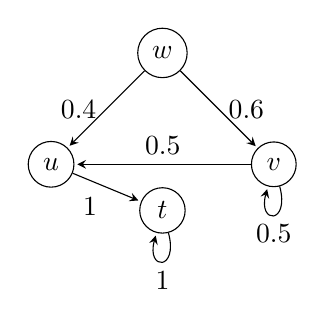
\begin{tikzpicture}[->,>=stealth,shorten >=1pt,auto,node distance=2cm]
        
        % Nodes
        \node[circle,draw] (w) {$w$};
        \node[circle,draw,below left of=w] (u) {$u$};
        \node[circle,draw,below right of=w] (v) {$v$};
        \node[circle,draw,below of=w] (t) {$t$};
        
        % Edges
        \path (w) edge node[left] {$0.4$} (u)
              (w) edge node[right] {$0.6$} (v)
              (u) edge node[below left] {$1$} (t)
              (v) edge node[above] {$0.5$} (u)
              (v) edge [loop below] node {$0.5$} (v)
              (t) edge [loop below] node {$1$} (t);
        
        \end{tikzpicture}
    \caption{Example of probabilistic Kripke model.}
    \label{fig:classic}
\end{figure}

Let $\prop=\{p,q\}$, we define a model $\model=(W,P,V)$ where  $W=\{u,v,w,t\}$, $P$ is the transition probability matrix depicted in Table~\ref{prob_matrix} and $V: \prop\rightarrow 2^W$ is defined such that $V(p)=\{u,w,t\}$ and $V(q)=\{v,t\}$.

\begin{table}[!ht]
    \centering
        \caption{Transition probability matrix of model depicted in Fig. \ref{fig:classic}.}
    \begin{tabular}{|c|c c c c|}
        \hline
         &$\quad u\quad$&$\quad v\quad$&$\quad w\quad$&$\quad t\quad$ \\\hline
         $\>u\>$&&&&1\\
         $v$&0.5 & 0.5&$\quad$&\\
         $w$& 0.4&0.6&&\\
         $t$& &&&1\\ \hline
    \end{tabular}
    \label{prob_matrix}
\end{table}

As an example, let us evaluate the formula $\Diamond_{0.5}(p \vee \Diamond_{0.8} \ q)$ at the state $w$:

\smallskip

$\M,w \models \Diamond_{0.5}(p \vee \Diamond_{0.8} \ q) \ \iff \ \displaystyle\sum_{\{x\in W \ \mid \ \M,x\models p \vee \Diamond_{0.8} \ q\}} P(w, x) \geq 0.5.$

Thus, for each state $x\in W$, we need to check whether $\model,x\models p \vee \Diamond_{0.8} \ q$, which holds if and only if $\model,x\models p$ or $\model,x\models \Diamond_{0.8} \ q$. Since $V(p)=\{u,w,t\}$, we only need to check the case $x=v$: 

$\model,v\models \Diamond_{0.8} \ q \ \iff \displaystyle\sum_{\{y \ \in W \ \mid \ \M,y\models \ q\}} P(v, y) \geq 0.8$.  According to the semantics, this is the case iff $P(v,v) + P(v,t) \geq 0.8$. But then we get $0.5 \geq 0.8$, which is false. \

Hence, $\displaystyle\sum_{\{x\in W \ \mid \ \M,x\models p \vee \Diamond_{0.8} \ q\}} P(w, x) \geq 0.5$ holds iff $P(w,w)+P(w,u) + P(w,t)\geq 0.5$, iff  $0.4 \geq 0.5$, which is false.

Therefore, $\M,w \not\models \Diamond_{0.5}(p \vee \Diamond_{0.8} \ q)$.

\end{example}


\subsection{Bisimulation}
%\textcolor{blue}{RF: the notions below are auto(bi)simulations. Is there a reason, or do we want it between two different models?}\textcolor{red}{It is not clear  how to define it. Here we have the condition of being a equivalence relation.} 
%\begin{definition}
%  Given a  probabilistic Kripke model  $\M=(S,P, V)$, a \emph{simulation} on $\M$ is an equivalence relation $B$ on $S$ such that it $s B s'$ we have
%  \begin{itemize}
%\item  $s\in V(p) $ iff $s'\in V(p) $
%\item for all $\displaystyle y\in S,  \sum_{w\in [y]} P(s,w) \leq\sum_{w\in [y]} P(s',w)$ %Find example of simulation that is not bisimulation
%\end{itemize}

%A bisimulation on $\M$ is an equivalence relation $B$ on $S$ such that it $s B s'$ we have
%\begin{itemize}
%\item  $s\in V(p) $ iff $s'\in V(p) $
%\item for all $\displaystyle y\in S,  \sum_{w\in [y]} P(s,w) =\sum_{w\in [y]} P(s',w)$
%\end{itemize}
%Being an equivalence relation can be dropped? 
  
%\end{definition}

%Two states are said to be probabilistically bisimilar if there is some such R relating them.

%\begin{theorem}
   % Given a  probabilistic Kripke model  $\M=(S,P, V)$ and  a \emph{simulation} on $\M$. Then for any $(w,w')\in B$ and any formula $\varphi$ we have $$\M,w \models \varphi \Longrightarrow \M,w' \models \varphi$$

%Moreover if  $B$ is a bisimulation we get  
    
 %$$\M,w \models \varphi \Longleftrightarrow \M,w' \models \varphi$$
    
%\end{theorem}

%NEW defintion

We now introduce a definition of bisimulation for the basic probabilistic case. While the classical definition usually defines bisimulation as an equivalence relation over the states of a probabilistic Kripke model, we introduce a version here to relate two different probabilistic Kripke models.

Probabilistic structures with labeled edges but without propositions are studied in~\cite{Panangaden2011}. In that paper, the author introduces the definition of dynamic relation based on the work in~\cite{BW01b,BW01a}, which does not require the relation to be an equivalence relation. Moreover, he proves that a dynamic relation implies the existence of a bisimulation relation. There, he was also able to prove the invariance and Hennessy-Milner theorem for finite models. Although that paper considers a probabilistic Kripke structure with labels, we use it as the basis for our definition within a context that also considers propositions.

\begin{definition}[Bisimulation]\label{bis} Let  $\M=(W,P, V)$ and  $\M' = (W', P', V')$ be two probabilistic Kripke models and $E \subseteq W \times W'$. We say that a nonempty relation $E$ is a \emph{bisimulation from $\M$ to $\M'$} if for every $w \in W$ and $w' \in W'$ such that $wEw'$, we have

\begin{description}
    \item[(atom):] for any $p \in \prop$, $w\in V(p)$ iff $w'\in V'(p)$,
    \item[(p-zigzag):] for any $U \subseteq W$, $\displaystyle \sum_{u \in U} P(w, u) \leq \displaystyle \sum_{u' \in E[U]} P'(w', u')$
\end{description}
\end{definition}

\begin{remark}
    Observe that the condition \textbf{(p-zigzag)} entails also its mirror condition \textbf{(p-zigzag')}. To prove this, let us consider a set $U'\subseteq W'$ and aiming for a contradiction assume that the following inequality holds:
    \begin{equation} \label{eq:zagzig}
        \displaystyle \sum_{u' \in U'} P'(w', u') > \displaystyle \sum_{ u  \in  E^{-1}[U']} P(w, u)
    \end{equation}
    We define $T := W \setminus E^{-1}[U']$ and observe that if $v'\in E[T]$ then $v'\notin U'$, so $U'$ and $E[T]$ are disjoint. 

    The condition \textbf{(p-zigzag)} for $T$ establishes that:
    \begin{equation} \label{eq:zigzag}
        \displaystyle \sum_{v \in T} P(w, v) \leq \displaystyle \sum_{ v' \in E[T]} P'(w', v')
    \end{equation}
    Now, combining equations \eqref{eq:zagzig} and \eqref{eq:zigzag} we get:
    \begin{multline}
        \label{eq:zagzig+zigzag}
        \displaystyle \sum_{v \in T} P(w, v) 
        +
        \displaystyle \sum_{ u \in E^{-1}[U']} P(w, u) <  
        \displaystyle \sum_{ v' \in E[T]} P'(w', v')
        +
        \displaystyle \sum_{u' \in U'} P'(w', u')
    \end{multline}
    Since $W = T \cup E^{-1} [U'] $, we have that:
    \begin{equation}
        \label{eq:first_part}
        \displaystyle \sum_{v \in T} P(w, v) 
        +
        \displaystyle \sum_{ u \in E^{-1}[U']} P(w, u)
        =
        1
    \end{equation}
    Based on the observation that $U'$ and $E[T]$ are disjoint, we can conclude that:
    \begin{equation}
        \label{eq:second_part}
        \displaystyle \sum_{ v' \in  E[T]} P'(w', v')
        +
        \displaystyle \sum_{u' \in U'} P'(w', u')
        \leq
        1
    \end{equation}
    Therefore, combining \eqref{eq:zagzig+zigzag}, \eqref{eq:first_part} and \eqref{eq:second_part} we get a contradiction.
\end{remark}

With this definition at hand, we are able to prove the following characterization result, usually called the \emph{invariance under bisimulation theorem}.

\begin{theorem}\label{th:inv_prob} Let  $\M=(W,P, V)$ and $\M' = (W', P', V')$ be two probabilistic Kripke models and $E \subseteq W \times W'$ a bisimulation from $\M$ to $\M'$. Then for any $(w,w')\in E$ and any formula $\varphi$ we have  $$\M,w \models \varphi \text{ iff } \M',w' \models \varphi$$
\end{theorem}

\begin{proof}
    The proof is obtained as a fragment of the proof of Theorem \ref{th:invariance}, that will be presented later on the paper.
\end{proof}
\section{Relation changing operators}\label{sec:prcml}

This section presents our main contribution, which is defining novel languages that extend probabilistic modal logic with a relation-changing modality, interpreted over probabilistic Kripke structures. The languages extend those in e.g.~\cite{ShiraziA07,ALDINI2024109167}. 
The `update' modality (written generally $\blacklozenge_{\sigma}$ here) will have two possible interpretations. First, as a sabotage-like modality (see~\cite{Fervari14,ArecesFH15,Aucher&vanBenthem&Grossi18})
in which the probability is subtracted from the edge accessing a chosen successor of the evaluation point, while it is transferred to another edge. Second, we introduce a bridge-like modality \cite{Fervari14,ArecesFH15}, in which the probability is instead taken from some edge to be added to the edge accessing the chosen successor. 

% Models are of the form $\model=(W,P,V)$, where $W$ is a set of states or worlds, $V:\prop \rightarrow 2^W$ is a standard valuation function, and $P:W\times W \times [0,1]$ and is such that for all $w\in W$, 
% \[
%     \sum_{w'\in W} P(w,w') = 1
% \]

The language we use is given by the following BNF:
\[
\varphi, \psi ::= p \mid \neg \varphi \mid \varphi \vee \psi \mid \Diamond_\rho \varphi \mid \blacklozenge_{\sigma} \varphi,
\]
where $p\in\prop$, $\rho \in [0,1]$ and $\sigma \in \ ]0,1[$. We denote the full set of formulas generated by the BNF above by $\form$. In the following, if the context is clear, we will use both $\Diamond_\rho$ and $\blacklozenge_\rho$.

The idea of changing a probabilistic relation implies that the transition probability matrix may change.  We define $Prob(W)$, the set of all transition probability matrices over the set $W$ as:
\[ 
    Prob(W)=\{P\in [0,1]^{W\times W}:\forall w\in W,\displaystyle\sum_{w' \in W} P(w, w') = 1\}.
\]

% In what follows, we will denote  by $\model , u \equiv_s \model' , u'$ whenever $\model , u \models \varphi$ iff $\model' , u' \models \varphi$ for all $\varphi \in \form $ with the sabotage semantics.


\subsection{Probabilistic Sabotage Operator}

Let us start by introducing the semantics of a local sabotage modality. In~~\cite{Fervari14,ArecesFH15}, a local sabotage is interpreted as moving the evaluation of the formula to a successor of the current point, while removing the traversed edge. In the graded/fuzzy case~\cite{FFM25}, edges have associated values, so the sabotage is carried out instead by reducing the value of the traversed edge. Here, we will follow a similar approach, but maintaining the properties of a probabilistic Kripke model.

\begin{definition}    
\label{def:sab-semantics}
Let $\M = (W, P, V)$ be a probabilistic Kripke structure, and let $w$ be a state in $W$. For any formula $\varphi\in\form$, we define 
the satisfaction relation $\models$ recursively as follows:
\[
    \begin{array}{l@{\ \ }c@{\ \ }l}
     \model,w\models p & \iff &  w\in V(p)\\ 
     \model,w\models\neg\varphi & \iff & \model,w\not\models\varphi \\         \model,w \models\varphi\vee\psi & \iff & \model,w\models\varphi \text{ or } \model,w\models\psi \\
    \model,w\models \Diamond_\rho \varphi & \iff &  \displaystyle\sum_{\{v \in W \mid  \model,v\models\varphi\}} P(w,v) \geq \rho \\
    \model,w\models \blacklozenge_\rho \varphi & \iff &  \text{exists } v\in W \mbox{ s.t. } \rho\leq \ P(w,v)\neq 1 , \mbox{ and } \model^{-(w,v)}_\rho, v \models\varphi, 
    \end{array}
\]

    % \begin{itemize}
    %     \item$\model,w\models p \mbox{ iff } w\in V(p)$;
    %     \item$\model\operatorname{val}(s, \lnot X) = \text{true} \ \text{iff} \ \operatorname{val}(s, X) = \text{false}$;
    %     \item$\model\operatorname{val}(s, X \land Y) = \text{true} \ \text{iff} \ \operatorname{val}(s, X) = \operatorname{val}(s, Y) = \text{true}$;
    %     \item $\model,w\models \Diamond_\rho \varphi \mbox{ iff } \Sigma_{(v \mid \model,v\models\varphi)} P(w,v) \geq \rho$;
    %      \item$\model,w\models \blacklozenge_\rho \varphi \mbox{ iff } \exists \ u,v\in W \mbox{ s.t. } u\neq v, \ P(w,v)\geq \rho, \mbox{ and } \model^{v-\rho}, v \models\varphi$.
    % \end{itemize}

\noindent where $\model^{-(w,v)}_\rho = (W, P^{-(w,v)}_\rho,V)$, with:
\begin{itemize}
    \item $P^{-(w,v)}_\rho(w,v)=P(w,v)-\rho$;
    \item $P^{-(w,v)}_\rho(w,t)=P(w,t)+\dfrac{\rho.P(w,t)}{1-P(w,v)}$, if  $ t \neq v$;
    \item $P^{-(w,v)}_\rho(s,t)=P(s,t)$, if $s\neq w$.
\end{itemize}

Note that  $\model^{-(w,v)}_\rho$ is a well-formed model, since it is updated in the context of the precondition $P(w,v)\geq \rho$ and, according to its definition, $P^{-(w,v)}_\rho\in Prob(W)$.
\end{definition}

In the rest of the paper, we will denote  by $\model , u \equiv_s \model' , u'$ whenever $\model , u \models \varphi$ iff $\model' , u' \models \varphi$ for all $\varphi \in \form $ with the sabotage semantics.

The semantic interpretation of the sabotage operator describes a scenario in which the probability of the event represented by an edge is reduced. When that is the case, the probability of the remaining ones (that also leave from the same origin state) is increased, in order to guarantee that the probability of all leaving edges sums to 1. For each of these edges, the increase is proportional to their pre-existing probability, so that the relative probabilities of the other positive outgoing transitions are preserved. This is illustrated in Example \ref{ex.sab}.

%Another question is, there exists a version of public announcements over this probabilistic logic with knowledge as in~\cite{ShiraziA07}?

\begin{example} \label{ex.sab}
Let us consider the model $(W,P,V)$ introduced in Example \ref{ex1}, and check if $w$ satisfies $\blacklozenge_{0.4} p$. By the semantics we have  
$\model,w\models\blacklozenge_{0.4} p$ iff $\exists x\in W$ s.t. $0.4\leq \ P(w,x)\neq 1$,  and $\model^{-(w,x)}_{0.4}, x \models p$.

$P(w,x)\geq 0.4$ implies $x=u$ or $x=v$. Although $v\not\in V(p)$, the formula is satisfied because $\model^{-(w,u)}_{0.4}, u \models p$. Moreover, the model $\model^{-(w,u)}_{0.4}=(W,P^{-(w,u)}_{0.4},V)$ is illustrated in Fig. \ref{fig:sabotage}.

\begin{figure}[!ht]
    \centering
        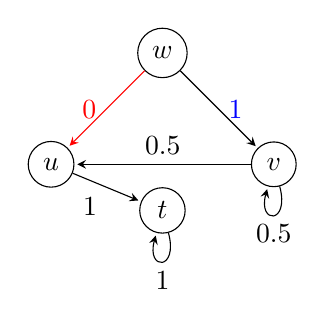
\begin{tikzpicture}[->,>=stealth,shorten >=1pt,auto,node distance=2cm]
        
        % Nodes
        \node[circle,draw] (w) {$w$};
        \node[circle,draw,below left of=w] (u) {$u$};
        \node[circle,draw,below right of=w] (v) {$v$};
        \node[circle,draw,below of=w] (t) {$t$};
        
        % Edges
        \path (w) edge[red] node[left,red] {$0$} (u)
              (w) edge node[right,blue] {$1$} (v)
              (u) edge node[below left] {$1$} (t)
              (v) edge node[above] {$0.5$} (u)
              (v) edge [loop below] node {$0.5$} (v)
              (t) edge [loop below] node {$1$} (t);
        
        \end{tikzpicture}
    \caption{The probabilistic Kripke model $(W,P^{-(w,u)}_{0.4},V)$.}
    \label{fig:sabotage}
\end{figure}
\end{example}

In general we will need to deal with nested updates over the original probability matrix $P$ of a model $\model$. Thus, we need to make sure that such a sequence of updates over $P$ leads to a well-formed probability matrix. We make these aspects precise in the following definition.

\begin{definition}[Sabotage well-formed]
    \label{def:sab-well-found}
    Let $\model=(W,P,V)$ be a probabilistic Kripke model. Let $\bar{\rho}=\rho_1,\dots,\rho_n$ and ${\overline{wv}}=(w_1,v_1),\ldots,(w_n,v_n)$ be two sequences such that $n\geq 0$, and for all $1\leq i \leq n$, $\rho_i\in]0,1]$ and $w_i,v_i\in W$. 
    
    For $0\leq k \leq n$,  $\bar{\rho}_k=\rho_1,\dots,\rho_k$ and ${\overline{wv}}_k=(w_1,v_1),\ldots(w_k,v_k)$ ($k=0$ yields empty sequences, denoted by $\varepsilon$). 
    We also define $\bar{\rho}\cdot \sigma=\rho_1,\dots,\rho_n,\sigma$ and ${\overline{wv}}\cdot(u,t)=(w_1,v_1),\ldots(w_k,v_k),(u,t)$, and define inductively $P^{-\overline{wv}}_{\bar{\rho}}$ as:
    $P_{\varepsilon}^{-\varepsilon}=P$ and $P_{\rho_k\cdot\sigma}^{-\overline{wv}\cdot (u,t)}= (P_{\rho_k}^{-\overline{wv}})^{-(u,t)}_\sigma$.

    Thus, we say that the updated matrix $P^{-\overline{wv}}_{\bar{\rho}}$ is \emph{well-formed (from $P$) for sabotage} if for all $0\leq j < n$, $\rho_{j+1} \leq P^{-{\overline{wv}}_j}_{\bar{\rho}_j}(w_{j+1},v_{j+1})\neq 1$. 
\end{definition}

\subsection{Probabilistic Bridge Operator}

Now it is time to move to the bridge case, generalizing~\cite{Fervari14,ArecesFH15}, and being more specific that in the graded case from~\cite{FFM25}. The idea is that if there no way to access some point with a certain probability value, the evaluation is moved to such a point, and the value is added to the traversed edge. This is similar to the graded case, but here we need to be careful to maintain the probability distribution. This is achieved by proportionally transferring the value from other edges to the intended one.

\begin{definition}
    
The satisfiability relation $\models$ is defined as in Def.~\ref{def:sab-semantics} for the Boolean cases and for $\Diamond_\rho$, and extended with the following case:
\[
    \begin{array}{l@{\ \ }c@{\ \ }l}
    %  \model,w\models p & \iff &  w\in V(p)\\ 
    %  \model,w\models\neg\varphi & \iff & \model,w\not\models\varphi \\         \model,w\models \varphi\vee\psi & \iff & \model,w\models\varphi \text{ or } \model,w\models\psi \\
    % \model,w\models \Diamond_\rho \varphi & \iff &  \displaystyle\sum_{\{v \in W \mid \model,v\models\varphi\}} P(w,v) \geq \rho \\
    \model,w\models \blacklozenge_\rho \varphi & \iff &  \text{exists } v\in W \mbox{ s.t. } \ P(w,v)+\rho\leq 1, \mbox{ and } \model^{+(w,v)}_\rho, v \models\varphi, 
    \end{array}
\]
    % \begin{itemize}
    %     \item$\model,w\models p \mbox{ iff } w\in V(p)$;
    %     \item$\model\operatorname{val}(s, \lnot X) = \text{true} \ \text{iff} \ \operatorname{val}(s, X) = \text{false}$;
    %     \item$\model\operatorname{val}(s, X \land Y) = \text{true} \ \text{iff} \ \operatorname{val}(s, X) = \operatorname{val}(s, Y) = \text{true}$;
    %     \item $\model,w\models \Diamond_\rho \varphi \mbox{ iff } \Sigma_{(v \mid \model,v\models\varphi)} P(w,v) \geq \rho$;
    %      \item$\model,w\models \blacklozenge_\rho \varphi \mbox{ iff } \exists \ u,v\in W \mbox{ s.t. } u\neq v, \ P(w,v)+\rho\leq 1, \mbox{ and } \model^{v+\rho}, v \models\varphi$.
    % \end{itemize}
where $\model^{+(w,v)}_\rho = (W, P^{+(w,v)}_\rho,V)$, with:
\begin{itemize}
    \item $P^{+(w,v)}_\rho(w,v)=P(w,v)+\rho$;
    %\textcolor{blue}{MAM: If $\rho> P(w,v)$?} \textcolor{red}{RF: this condition is taken care in the  precondition of the modality. It depends how we want to define it.MAM: OK}
    \item $P^{+(w,v)}_\rho(w,t)=P(w,t)-
\dfrac{\rho.P(w,t)}{1-P(w,v)}$, if $ t \neq v$;
    \item $P^{+(w,v)}_\rho(s,t)=P(s,t)$, if $s\neq w$.
\end{itemize}

Again, note that $\model^{+(w,v)}_\rho$ is a well-formed model.

In what follows, we will denote  by $\model , u \equiv_b \model' , u'$ whenever $\model , u \models \varphi$ iff $\model' , u' \models \varphi$ for all $\varphi \in \form $ with the bridge semantics.

\end{definition}

The semantics of the bridge operator depicts a case where either the probability of an event to occur increases or some new transition is possible. Thus, the probability assigned to the other edges that also leave from the same origin state must decrease. As in the case of the ``sabotage'', this reduction is obtained in a proportional way, based on the previous value of each edge probability. This is illustrated in Example \ref{ex:brid}.

\begin{example}\label{ex:brid}
Let us recall the model $(W,P,V)$ from Example \ref{ex1} and check if $v$ satisfies $\blacklozenge_{0.4} q$. By the semantics we have 
$\model,v\models\blacklozenge_{0.4} q$ iff $\exists x\in W$ s.t. $0.4\leq \ P(v,x)\neq 1$,  and $\model^{+(v,x)}_{0.4}, x \models q$.

$P(v,x)\leq 0.4$ implies $x=w$ or $x=t$. Although $w\not\in V(p)$, the formula is satisfied because $\model^{+(v,t)}_{0.4}, t \models p$. Moreover, the model $\model^{+(v,t)}_{0.4}=(W,P^{+(v,t)}_{0.4},V)$ is illustrated in Fig. \ref{fig:bridge}.

\begin{figure}[!ht]
    \centering
        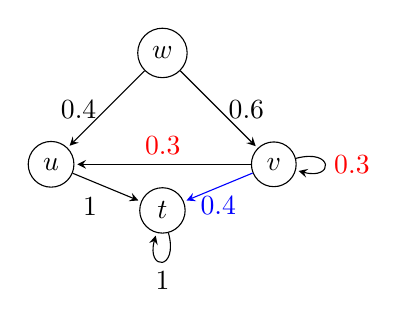
\begin{tikzpicture}[->,>=stealth,shorten >=1pt,auto,node distance=2cm]
        
        % Nodes
        \node[circle,draw] (w) {$w$};
        \node[circle,draw,below left of=w] (u) {$u$};
        \node[circle,draw,below right of=w] (v) {$v$};
        \node[circle,draw,below of=w] (t) {$t$};
        
        % Edges
        \path (w) edge node[left] {$0.4$} (u)
              (w) edge node[right] {$0.6$} (v)
              (u) edge node[below left] {$1$} (t)
              (v) edge node[above,red] {$0.3$} (u)
              (v) edge [loop right] node[red] {$0.3$} (v)
              (v) edge [below,blue] node[blue] {$0.4$} (t)
              (t) edge [loop below] node {$1$} (t);
        
        \end{tikzpicture}
    \caption{The probabilistic Kripke model $(W,P^{+(v,t)}_{0.4},V)$.}
    \label{fig:bridge}
\end{figure}
\end{example}

Again, we need to establish when a sequence of updates is well-formed.

\begin{definition}[Bridge well-formed]
    \label{def:bridge-well-found}
    Let $\model=(W,P,V)$, $\bar{\rho}=\rho_1,\dots,\rho_n$ and ${\overline{wv}}=(w_1,v_1),\ldots,(w_n,v_n)$ as in Def.~\ref{def:sab-well-found}. Let $P^{+\overline{wv}}_{\bar{\rho}}$
    be defined analogously to~$P^{-\overline{wv}}_{\bar{\rho}}$. 
    % For $0\leq k \leq n$,  $\bar{\rho}_k=\rho_1,\dots,\rho_k$ and ${\overline{wv}}_k=(w_1,v_1),\ldots(w_k,v_k)$ ($k=0$ yields empty sequences $\varepsilon$). 
    % We also define $\bar{\rho}\cdot \sigma=\rho_1,\dots,\rho_n,\sigma$ and ${\overline{wv}}\cdot(u,t)=(w_1,v_1),\ldots(w_k,v_k),(u,t)$, and define inductively $P^{-\overline{wv}}_{\bar{\rho}}$ as:
    % $P_{\varepsilon}^{-\varepsilon}=P$ and $P_{\rho_k\cdot\sigma}^{-\overline{wv}\cdot (u,t)}= (P_{\rho_k}^{-\overline{wv}})^{-(u,t)}_\sigma$.

    We say that the updated matrix $P^{+\overline{wv}}_{\bar{\rho}}$ is \emph{well-formed (from $P$) for bridge} if for all $0\leq j < n$, $ P^{+{\overline{wv}}_j}_{\bar{\rho}_j}(w_{j+1},v_{j+1}) + \rho_{j+1}\leq 1$. 
\end{definition}

\subsection{Probabilistic Swap Operator}

We conclude this section by introducing a local swap modality, inspired by~\cite{ArecesFH14}. In a non-probabilistic setting, a swap modality can be seen as a double operation in which we remove an edge $(w,v)$ and we add its converse edge $(v,w)$. We can mimic this behaviour here, by taking both the precautions as in the sabotage and bridge: once some value $\rho$ is decreased between a node $w$ and $v$, we need to make sure that such a value is reassigned to the rest of successors of $w$. But also, since the value $\rho$ is increased from $v$ to $w$, now we need to remove such a value from $v$-successors proportionally. We formalize this idea in the semantics definition below.

\begin{definition}
    \label{def:swap-semantics}
    The satisfiability relation $\models$ is defined as in Def.~\ref{def:sab-semantics} for the Boolean cases and for $\Diamond_\rho$, and extended with the following case:
\[
    \begin{array}{l@{\ \ }c@{\ \ }l}
    %  \model,w\models p & \iff &  w\in V(p)\\ 
    %  \model,w\models\neg\varphi & \iff & \model,w\not\models\varphi \\         \model,w\models \varphi\vee\psi & \iff & \model,w\models\varphi \text{ or } \model,w\models\psi \\
    % \model,w\models \Diamond_\rho \varphi & \iff &  \displaystyle\sum_{\{v \in W \mid \model,v\models\varphi\}} P(w,v) \geq \rho \\
    \model,w\models \blacklozenge_\rho \varphi & \iff & \text{there exists }v\in W\text{ s.t. } \\
    && \rho \leq P(w,v)\neq 1,\quad P(v,w)+\rho\leq 1 \text{ and }\model^{*(w,v)}_\rho, v \models\varphi,
    \end{array}
\]
    % \begin{itemize}
    %     \item$\model,w\models p \mbox{ iff } w\in V(p)$;
    %     \item$\model\operatorname{val}(s, \lnot X) = \text{true} \ \text{iff} \ \operatorname{val}(s, X) = \text{false}$;
    %     \item$\model\operatorname{val}(s, X \land Y) = \text{true} \ \text{iff} \ \operatorname{val}(s, X) = \operatorname{val}(s, Y) = \text{true}$;
    %     \item $\model,w\models \Diamond_\rho \varphi \mbox{ iff } \Sigma_{(v \mid \model,v\models\varphi)} P(w,v) \geq \rho$;
    %      \item$\model,w\models \blacklozenge_\rho \varphi \mbox{ iff } \exists \ u,v\in W \mbox{ s.t. } u\neq v, \ P(w,v)+\rho\leq 1, \mbox{ and } \model^{v+\rho}, v \models\varphi$.
    % \end{itemize}
where $\model^{*(w,v)}_\rho = (W, P^{*(w,v)}_\rho,V)$, with:
\begin{itemize}
    \item $P^{*(w,v)}_\rho(w,v)=P(w,v)-\rho$;
    \item $P^{*(w,v)}_\rho(v,w)=P(v,w)+\rho$;
    \item $P^{*(w,v)}_\rho(w,t)=P(w,t)+
\dfrac{\rho.P(w,t)}{1-P(w,v)}$, if $ t \neq v$;
    \item $P^{*(w,v)}_\rho(v,t)=P(v,t)-
\dfrac{\rho.P(v,t)}{1-P(v,w)}$, if $ t \neq w$;
    \item $P^{*(w,v)}_\rho(s,t)=P(s,t)$, if $v\neq s\neq w$.
\end{itemize}

Again, note that $\model^{*(w,v)}_\rho$ is a well-formed model.

In what follows, we will denote  by $\model , u \equiv_w \model' , u'$ whenever $\model , u \models \varphi$ iff $\model' , u' \models \varphi$ for all $\varphi \in \form $ with the swap semantics.

\end{definition}

Again, we need to establish when a sequence of updates is well-formed.

\begin{definition}[Swap well-formed]
    \label{def:swap-well-found}
    Let $\model=(W,P,V)$, $\bar{\rho}=\rho_1,\dots,\rho_n$ and ${\overline{wv}}=(w_1,v_1),\ldots,(w_n,v_n)$ as in Def.~\ref{def:sab-well-found}. Let $P^{*\overline{wv}}_{\bar{\rho}}$
    be defined analogously to~$P^{-\overline{wv}}_{\bar{\rho}}$. 
    % For $0\leq k \leq n$,  $\bar{\rho}_k=\rho_1,\dots,\rho_k$ and ${\overline{wv}}_k=(w_1,v_1),\ldots(w_k,v_k)$ ($k=0$ yields empty sequences $\varepsilon$). 
    % We also define $\bar{\rho}\cdot \sigma=\rho_1,\dots,\rho_n,\sigma$ and ${\overline{wv}}\cdot(u,t)=(w_1,v_1),\ldots(w_k,v_k),(u,t)$, and define inductively $P^{-\overline{wv}}_{\bar{\rho}}$ as:
    % $P_{\varepsilon}^{-\varepsilon}=P$ and $P_{\rho_k\cdot\sigma}^{-\overline{wv}\cdot (u,t)}= (P_{\rho_k}^{-\overline{wv}})^{-(u,t)}_\sigma$.

    We say that the updated matrix $P^{*\overline{wv}}_{\bar{\rho}}$ is \emph{well-formed (from $P$) for swap} if for all $0\leq j < n$, $\rho_{j+1}\leq P^{*{\overline{wv}}_j}_{\bar{\rho}_j}(w_{j+1},v_{j+1})\neq 1$ and $P^{*{\overline{wv}}_j}_{\bar{\rho}_j}(v_{j+1},w_{j+1})+\rho_{j+1}\leq 1$. 
\end{definition}
\section{Probabilistic Relation-Changing Bisimulations}
\label{sec:bisimulation}

\subsection{Bisimulations}
\label{sec:bisimdef}

Based on Def.~\ref{bis}, we introduce a notion of bisimulation for the probabilistic language obtained by adding either of our relation-changing operators: sabotage, bridge or swap. 

\begin{definition}[Bisimulation] \label{switch_bis} Let  $\M=(W,P, V)$ and  $M' = (W', P', V')$ be two probabilistic Kripke models. % and $E \subseteq \big(W\times Prob(W)\big) \times \big(W'\times Prob(W')\big)$ . 
We say that a non-empty relation $E\subseteq \big(W\times Prob(W)\big) \times \big(W'\times Prob(W')\big)$ is a $\rho$-sabotage \emph{bisimulation from $\M$ to $\M'$} if, for every pair $\big((w,Q) ,(w',Q')\big)\in E$, the following holds:

\begin{description}


\item[\textbf{(atom)}:] $w\in V(p)$ iff $w'\in V'(p)$, for all $p\in\prop$;

\item [\textbf{(p-zigzag)}:] for any $U \subseteq W$, $\displaystyle \sum_{u \in U} Q(w, u) \leq \displaystyle \sum_{ (u',Q') \ \in \ \bigcup_{u\in U}E[(u,Q)]} Q'(w', u')$;

%\item [$\mathbf{zag_{prob}:}$] for any $U' \subseteq W'$, $\displaystyle \sum_{u' \in U'} P'(w', u') \leq \displaystyle \sum_{(u,P)\in \bigcup_{u'\in U'}E^{-1}[(u',P')]} P(w, u)$;

% \item [\textbf{(sab-zig)}:] for any $u \in W$ s.t. $1\neq P(w, u)>\rho$, exists $u'\in W'$ such that:
%     \begin{enumerate}
%         \item $P(w, u) \leq P'(w', u')<1$, and 
%         \item $\big(u,P^{-(w,u)}_{\rho}\big)E\big(u',P'^{-(w',u')}_{\rho}\big)$;
%     \end{enumerate}
\item [\textbf{(sab-zig)}:] for any $u\in W$ s.t. $\rho\le Q(w,u)\neq 1$, there is $u'\in W'$ s.t.    
\begin{enumerate}
    \item $\rho\le Q'(w',u')\neq 1$ and 
    \item $(u,Q_\rho^{-(w,u)})E(u',Q'^{-(w',u')}_\rho)$.  
\end{enumerate}
\item [\textbf{(sab-zag)}:] for any $u'\in W'$ s.t. $\rho\le Q'(w',u')\neq 1$, there is $u\in W$ s.t.    
\begin{enumerate}
    \item $\rho\le Q(w,u)\neq 1$ and 
    \item $(u,Q_\rho^{-(w,u)})E(u',Q'^{-(w',u')}_\rho)$.  
\end{enumerate}
%
% \item [\textbf{(sab-zag)}:] for any $u' \in W'$ s.t. $1\neq P'(w', u')>\rho$, exists $u\in W$ such that: 
%     \begin{enumerate}
%         \item $P'(w', u') \leq P(w, u)<1$, and 
%         \item $\big(u,P^{-(w,u)}_{\rho}\big)E\big(u',P'^{-(w',u')}_{\rho}\big)$.
%     \end{enumerate}
\end{description}

We say that $E$ is a $\rho$-bridge \emph{bisimulation from $\M$ to $\M'$} if, for every pair $\big((w,Q) ,(w',Q')\big)\in E$, \textbf{(atom)}, \textbf{(p-zigzag)} above and the following holds:

\begin{description}
    % \item [\textbf{(br-zig)}:] for any $u \in W$ s.t. $P(w, u)+\rho<1$, exists $u'\in W'$ such that:
    % \begin{enumerate}
    %     \item $P(w, u) \geq P'(w', u')$, and 
    %     \item $\big(u,P^{+(w,u)}_{\rho}\big)E\big(u',P'^{+(w',u')}_{\rho}\big)$;
    % \end{enumerate} 
    \item[(br-zig):]  for any $u\in W$ s.t. $Q(w,u)+\rho\le 1$, there is $u'\in W'$ s.t.
        \begin{enumerate}
            \item $Q'(w',u')+\rho\le 1$ and 
            \item $(u,Q_\rho^{+(w,u)})\,E\,(u',Q'^{+(w',u')}_\rho)$.
        \end{enumerate}
    
    \item[(br-zag):]  for any $u'\in W'$ s.t. $Q'(w',u')+\rho\le 1$, there is $u\in W$ s.t.
        \begin{enumerate}
            \item $Q(w,u)+\rho\le 1$ and 
            \item $(u,Q_\rho^{+(w,u)})\,E\,(u',Q'^{+(w',u')}_\rho)$.
        \end{enumerate}

    % \item [\textbf{(br-zag)}:] for any $u' \in W'$ s.t. $P'(w', u')+\rho<1$, exists $u\in W$ such that: 
    % \begin{enumerate}
    %     \item $P'(w', u') \geq P(w, u)$ and 
    %     \item $\big(u,P^{+(w,u)}_{\rho}\big)E\big(u',P'^{+(w',u')}_{\rho}\big)$.
    % \end{enumerate}

    % \item[\textbf{(univ):}] for all $w\in W, w'\in W'$, $E[\{(w,P)\}]\neq \emptyset \neq E^{-1}[\{(w',P')\}]$.
\end{description}

Finally, we say that $E$ is a $\rho$-swap \emph{bisimulation from $\M$ to $\M'$} if, for every pair $\big((w,Q) ,(w',Q')\big)\in E$, \textbf{(atom)}, \textbf{(p-zigzag)} above and the following holds:

\begin{description}
    % \item [\textbf{(sw-zig)}:] for any $u \in W$ s.t. $\rho < P(w, u) \neq 1$ and $P(u,w) + \rho < 1$, exists $u'\in W'$ such that:
    % \begin{enumerate}
    %     \item $P(w, u) \leq P'(w', u') < 1$, 
    %     \item $P(u, w) \geq P'(u', w')$, and 
    %     \item $\big(u,P^{*(w,u)}_{\rho}\big)E\big(u',P'^{*(w',u')}_{\rho}\big)$;
    % \end{enumerate} 

    \item[(sw-zig):]  for any $u\in W$ s.t. $\rho\le Q(w,u)\neq 1$ and $Q(u,w)+\rho\le 1$, there is $u'\in W'$ s.t. 
        \begin{enumerate}
            \item $\rho\le Q'(w',u')\neq 1$, $Q'(u',w')+\rho\le 1$ and
            \item $(u,Q_\rho^{*(w,u)})\,E\,(u',Q'^{*(w',u')}_\rho)$.
        \end{enumerate}

    \item[(sw-zag):]  for any $u'\in W'$ s.t. $\rho\le Q'(w',u')\neq 1$ and $P(u',w')+\rho\le 1$, there is $u\in W$ s.t. 
        \begin{enumerate}
            \item $\rho\le Q(w,u)\neq 1$, $Q(u,w)+\rho\le 1$ and
            \item $(u,Q_\rho^{*(w,u)})\,E\,(u',Q'^{*(w',u')}_\rho)$.
        \end{enumerate}
    % \item [\textbf{(sw-zag)}:] for any $u' \in W'$ s.t. $\rho < P'(w', u') \neq 1$ and $P'(u', w')+\rho<1$, exists $u\in W$ such that: 
    % \begin{enumerate}
    %     \item $P'(w', u') \leq P(w, u) < 1$, 
    %     \item $P'(u', w') \geq P(u, w)$ and 
    %     \item $\big(u,P^{*(w,u)}_{\rho}\big)E\big(u',P'^{*(w',u')}_{\rho}\big)$.
    % \end{enumerate}
    
\end{description}


% \noindent In addition, for $\rho$-bridge bisimulation, we also impose that for all $w\in W, w'\in W'$, $E[\{(w,P)\}]\neq \emptyset \neq E^{-1}[\{(w',P')\}]$.

We say that $E$ is a sabotage bisimulation (resp. bridge/swap bisimulation) if it is a $\rho$-sabotage  (resp. $\rho$-bridge/$\rho$-swap) bisimulation for every $\rho\in]0,1[$. Moreover, if $E$ is a bisimulation and $(w,P) E  (w',P')$, we say that $w$ and $w'$ are two sabotage (resp. bridge/swap) bisimilar states.
\end{definition}

We note that our definitions of relation-changing bisimulations do not fully generalize the classical one. However, this is indeed caused by the semantic interpretation of the new operator $\blacklozenge_\rho$ under the different semantics, that can distinguish two probabilistic Kripke models such as the ones illustrated in Fig.~\ref{ex_not_bis}, which are bisimilar according to the classical definition. Thus, contrary to the classical case, we need to consider both \textbf{(sab-zig)}/\textbf{(br-zig)}/\textbf{(sw-zig)} and \textbf{(sab-zag)}/\textbf{(br-zag)}/\textbf{(sw-zag)}  conditions. As it is possible to note in Fig.~\ref{ex_not_bis}, the \textbf{(sab-zig)},  \textbf{(br-zig)} and \textbf{(sw-zig)} conditions are verified from left to right model, but not in the opposite direction.

\begin{figure}
    \centering
        \begin{minipage}{0.48\linewidth}
        \centering
            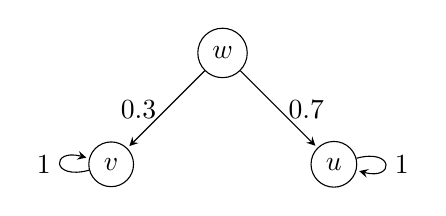
\begin{tikzpicture}[->,>=stealth,shorten >=1pt,auto,node distance=2cm]
        
        % Nodes
        \node[circle,draw] (w) {$w$};
        \node[circle,draw,below left of=w] (v) {$v$};
        \node[circle,draw,below right of=w] (u) {$u$};
        
        % Edges
        \path (w) edge node[left] {$0.3$} (v)
              (w) edge node[right] {$0.7$} (u)
              (u) edge [loop right] node {$1$} (v)
              (v) edge [loop left] node {$1$} (v);
        
        \end{tikzpicture}
        \end{minipage}\begin{minipage}{0.48\linewidth}
        \centering
            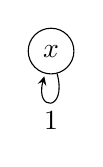
\begin{tikzpicture}[->,>=stealth,shorten >=1pt,auto,node distance=2cm]
        
        % Nodes
        \node[circle,draw] (x) {$x$};
        
        % Edges
        \path (x) edge [loop below] node {$1$} (x);
        
        \end{tikzpicture}
        \end{minipage}
    \caption{Two models whose states are bisimilar but not sabotage/bridge/swap bisimilar.}
    \label{ex_not_bis}
\end{figure}

\subsection{Invariance Theorems for Probabilistic Relation-Changing Modalities}
\label{sec:invariance}

In this section we will start by proving that the notions of bisimulation we just introduced, are adequate for the respective logic. Our first result concerns a minimal condition we aim to satisfy, namely that two probabilistic models that are bisimilar for some of the notions from previous section, satisfy the same set of formulas of the respective logic. 

\begin{theorem}[Invariance]\label{th:invariance}
    Let $\model=(W,P,V)$ and $\model'=(W',P',V')$ be two probabilistic Kripke models and let $E\subseteq \big((W\times Prob(W)\big) \times \big(W'\times Prob(W')\big)$ be a sabotage (resp. bridge/swap) bisimulation. Then, $(w,P)E(w',P')$ implies $\model,w\equiv_{\mathsf{sb}}\model',w'$ (resp. $\model,w\equiv_{\mathsf{br}}\model',w'$/$\model,w\equiv_{\mathsf{sw}}\model',w'$).
\end{theorem}

\begin{proof}
    We prove the theorem by induction over the structure of formulas. Moreover, we will prove a more general result: for all well-formed matrices ${Q}$ and ${Q'}$, $(w,{Q})E(w',{Q}')$ implies $(W,{Q},V),w\equiv_{\mathsf{sb}}(W',{Q}',V'),w'$.  
    We firstly consider the sabotage semantics.
    
    \medskip
    \noindent \underline{Base case:}
    \begin{itemize}
        \item If $\varphi\in\prop$, then the result follows from \textbf{(atom)}  from Def. \ref{switch_bis}.
    \end{itemize}
    
    \noindent \underline{Inductive cases:}
    \begin{itemize}
        \item If $\varphi=\neg\psi$, then $(W,{Q},V),w\models\neg\psi$ iff $(W,{Q},V),w\not\models\psi$. By IH, $(W',{Q}',V'),w'\not\models\psi$, and then 
        $(W',{Q}',V'),w'\models\neg\psi$.

        \item If $\varphi=\psi\vee\chi$, then $(W,{Q},V),w\models\psi\vee\chi$ iff, by definition, $(W,{Q},V),w\models\psi$ or $(W,{Q},V),w\models\chi$. Thus, by IH, we obtain that $(W',{Q}',V'),w'\models\psi$ or $(W',{Q}',V'),w'\models\chi$, hence $(W',{Q}',V'),w'\models\psi\vee\chi$.

        \item If $\varphi=\Diamond_\rho \psi$, then $(W,{Q},V),w\models \Diamond_\rho \psi$ iff $\sum_{\{v \in W \mid (W,{Q},V),v\models\psi\}} {Q}(w,v) \geq \rho$. Note that (by Def.~\ref{switch_bis}) 

        \[
            \begin{aligned}
            & \sum_{\{v\in W \mid (W,{Q},V),v\models\psi\}} {Q}(w,v) \\
            \leq & \sum_{\{v'\in W' \mid  (v',{Q}')\in \bigcup_{\{v \in W \ \mid \ (W,{Q},V),v\models\psi\}}E[(v,{Q})]\}} {Q}'(w',v') \\ 
            \leq & \sum_{\{v' \in W' \mid  (W',{Q}',V'),v'\models\psi\}} {Q}'(w',v')
            \end{aligned}    
        \]
        (since $(v,{Q})E(v',{Q}')$, and by IH). Moreover, by using the same reasoning we can conclude that
        \[
            \begin{aligned}
            \sum_{\{v \in W \mid  (W,{Q},V),v\models\neg\psi\}}{Q}(w,v) &\leq 
            \sum_{\{v' \in W' \mid (W',{Q}',V'),v'\models\neg\psi)\}} {Q}'(w',v').
            \end{aligned}
        \]
        Since for all $w\in W$, $\sum_{v \in W}{Q}(w,v)=1$ and for all $w'\in W'$,  it holds that $\sum_{v' \in W'}{Q}(w',v')=1$, we get  
        \[
            \sum_{\{v\in W \ \mid \ (W,{Q},V),v\models\psi\}}{Q}(w,v)= \sum_{\{v' \in W' \mid (W',{Q}',V'),v'\models\psi\}} {Q}'(w',v'),
        \]  
        because every $w\in W\cup W'$  satisfies either $\psi$  or $\neg\psi$. 
        Hence, we can conclude $(W,{Q},V),w\models \Diamond_\rho \psi$ iff 
        $(W',{Q}',V'),w'\models \Diamond_\rho \psi$.

        % \item If $\varphi= \blacklozenge_\rho \psi$, then $(W,{Q},V),w\models \blacklozenge_\rho \psi$ iff exists  $v\in W$ s.t.  $\rho\leq {Q}(w,v) < 1$,  and  $(W,{Q}^{-(w,v)}_\rho,V), v \models\psi$. From \textbf{(sab-zig)} in Def.~\ref{switch_bis}, there exists $v'\in W'$ s.t. ${Q}(w,v)\leq {Q}'(w',v') < 1$  and $(v,{Q}^{-(w,v)}_\rho)E(v',{Q}'^{-(w',v')}_\rho)$. Thus, by IH, exists $v'\in W'$, s.t. $\rho\leq {Q}'(w',v')<1$, and $(W',{Q}'^{-(w',v')}_\rho,V'), v' \models\psi$, and therefore $(W',{Q}',V'), w'\models\blacklozenge_\rho\psi$.
        \item Suppose $\varphi= \blacklozenge_\rho \psi$ and $(W,{Q},V),w\models \blacklozenge_\rho \psi$. Then, there exists  $v\in W$ such that  $\rho\leq {Q}(w,v) < 1$,  and  $(W,{Q}^{-(w,v)}_\rho,V), v \models\psi$. From \textbf{(sab-zig)} in Def.~\ref{switch_bis}, there exists $v'\in W'$ such that $\rho\leq {Q}'(w',v') \neq 1$  and $(v,{Q}^{-(w,v)}_\rho)E(v',{Q}'^{-(w',v')}_\rho)$. Thus, by IH, exists $v'\in W'$, s.t. $\rho\leq {Q}'(w',v')<1$, and $(W',{Q}'^{-(w',v')}_\rho,V'), v' \models\psi$, and therefore, we conclude that $(W',{Q}',V'), w'\models\blacklozenge_\rho\psi$.

        The reciprocal implication is proved analogously, using \textbf{(sab-zag)}.
    \end{itemize}

    Therefore, since $P$ and $P'$ are well-formed and they are s.t. $(w,P)E(w',P')$, we can conclude that $\model,w\equiv_{\mathsf{sb}}\model',w'$.
    
    %$\model,w\models \blacklozenge_\rho \varphi$ \ iff \ $\exists \ v\in W \mbox{ s.t. }  \ P(w,v)\geq \rho, \mbox{ and } \model^{-(w,v)}_\rho, v \models\varphi$

   % By definition of bisimulation, $\exists \ v'\in W'$ s.t. $(w',u')\in E$ and $P'(w',v')=P(w,v)$. Also, Lemma \ref{lemma} guarantees that $E$ is still a bisimulation between $\model^{-(w,v)}_\rho$ and $\model'^{-(w',v')}_\rho$. Thus, by induction hypothesis, we deduct:

    %$\exists \ v'\in W' \mbox{ s.t. }  \ P'(w',v')\geq \rho, \mbox{ and } \model^{-(w',v')}_\rho, v' \models\varphi$ iff $\model',w'\models \blacklozenge_\rho \varphi$

   % The opposite implication is proved analogously.
    The result for bridge semantics is obtained using the analogous reasoning. We prove only the case for formulas with the $\blacklozenge$ modality:

    % \begin{itemize}
    %     \item Suppose $\varphi=\blacklozenge_\rho\psi$ and $(W,{Q},V),w\models\blacklozenge_\rho\psi$. Then there is $v\in W$ such that
    %         ${Q}(w,v)+\rho\leq 1
    %         \quad\text{and}\quad
    %         (W,{Q}^{+(w,v)}_\rho,V),v\models\psi$. 
    %     By \textbf{(br-zig)} in Def.~\ref{switch_bis}, there exists $v'\in W'$ such that
    %     \[
    %         {Q}(w,v')\geq{Q}'(w',v')
    %         \quad\text{and}\quad
    %         (v,{Q}^{+(w,v)}_\rho)E(v',{Q}'^{+(w',v')}_\rho).
    %     \]
    %     Therefore,
    %     \[
    %         {Q}'(w',v')+\rho
    %         \leq{Q}(w,v')+\rho
    %         \leq 1.
    %     \]
    %     By the induction hypothesis,
    %     \[
    %         (W',{Q}'^{+(w',v')}_\rho,V'),v'\models\psi.
    %     \]
    %     Therefore,
    %     \[
    %         (W',{Q}',V'),w'\models\blacklozenge_\rho\psi.
    %     \]
    % \end{itemize}
 \begin{itemize}
        \item Suppose $\varphi=\blacklozenge_\rho\psi$ and $(W,{Q},V),w\models\blacklozenge_\rho\psi$. Then, there is $v\in W$ such that
            ${Q}(w,v)+\rho\leq 1$ and $(W,{Q}^{+(w,v)}_\rho,V),v\models\psi$. 
        By \textbf{(br-zig)} in Def.~\ref{switch_bis}, there exists $v'\in W'$ s.t. 
        ${Q}'(w',v') + \rho \leq 1$ and $(v,{Q}^{+(w,v)}_\rho)E(v',{Q}'^{+(w',v')}_\rho)$. 
        % Therefore,
        % \[
        %     {Q}'(w',v')+\rho
        %     \leq{Q}(w,v')+\rho
        %     \leq 1.
        % \]
        By IH, we get $(W',{Q}'^{+(w',v')}_\rho,V'),v'\models\psi$. 
        Therefore, we can conclude $(W',{Q}',V'),w'\models\blacklozenge_\rho\psi$. 
    \end{itemize}
    The reciprocal implication is obtained analogously by using \textbf{(br-zag)}.


    It remains the verify that the result also holds under swap semantics:
    \begin{itemize}
            \item Suppose $\varphi=\blacklozenge_\rho\psi$ and $(W,{Q},V),w\models\blacklozenge_\rho\psi$. Then, there exists $v\in W$ such that
                $\rho \leq {Q}(w,v) \neq 1$, 
                ${Q}(v,w)+\rho\leq 1$, and
                $(W,{Q}^{*(w,v)}_\rho,V),v\models\psi$. 
            By \textbf{(sw-zig)} in Def.~\ref{switch_bis}, there exists $v'\in W'$ such that
               $\rho\le Q'(w',u')\neq 1$, $Q'(u',w')+\rho\le 1$ 
                and 
                $(v,{Q}^{*(w,v)}_\rho)E(v',{Q}'^{*(w',v')}_\rho)$. 
            Thus, by IH, we obtain 
            $(W',{Q}'^{*(w',v')}_\rho,V'),v'\models\psi$. 
            Therefore, 
                $(W',{Q}',V'),w'\models\blacklozenge_\rho\psi$.
        \end{itemize}
         Once again, the reciprocal implication is obtained using \textbf{(sw-zag)}.
    % \begin{itemize}
    %     \item Suppose $\varphi=\blacklozenge_\rho\psi$ and $(W,{Q},V),w\models\blacklozenge_\rho\psi$. Then there is $v\in W$ such that
    %     \begin{itemize}
    %         \item $\rho \leq {Q}(w,v) \neq 1$, 
    %         \item ${Q}(v,w)+\rho\leq 1$, and
    %         \item $(W,{Q}^{*(w,v)}_\rho,V),v\models\psi$.
    %     \end{itemize}
    %     By \textbf{(sw-zig)} in Def.~\ref{switch_bis}, there exists $v'\in W'$ such that
    %     \begin{itemize}
    %         \item ${Q}(w,v) \leq {Q}'(w',v') < 1$, 
    %         \item ${Q}'(v',w') \leq {Q}(v,w) $, and
    %         \item $(v,{Q}^{*(w,v)}_\rho)E(v',{Q}'^{*(w',v')}_\rho)$.
    %     \end{itemize}
    %     Then,
    %     \begin{itemize}
    %         \item $\rho \leq {Q}(w,v) \leq {Q}'(w',v') < 1$, and 
    %         \item ${Q}'(v',w') + \rho \leq {Q}(v,w) + \rho \leq 1$.
    %     \end{itemize}
    %     By IH,
    %     \[
    %         (W',{Q}'^{*(w',v')}_\rho,V'),v'\models\psi.
    %     \]
    %     Therefore,
    %     \[
    %         (W',{Q}',V'),w'\models\blacklozenge_\rho\psi.
    %     \]
    % \end{itemize}
    %Here we note that the additional condition \textbf{(univ)} (i.e., for all $w\in W$,  $w'\in W'$, $E[\{(w,P)\}]\neq \emptyset \neq E^{-1}[\{(w',P')\}]$)  ensures that it is not possible to create a bridge to a new state that was not previously bisimilar to any other. This is not required for sabotage because the probability assigned to edges with probability of $0$ is never changed.
\end{proof}

%$Prob(W)$ is the set of all probabilistic matrices $W\times W$

%\textcolor{red}{The generalization of bisimulation is not straightforward}
%\begin{definition}[Bridge-bisimulation]
 %   Given a  probabilistic Kripke model  $\M=(S,P, V)$, a \emph{bisimulation} on $\M$ is an equivalence relation $B$ on $S$ such that it $s B s'$ we have
 
 %   A relation $Z\subseteq (W \times Prob(W) \times (W'\times Prob(W))$ is a \emph{bridge bisimulation} if and only if, $(w,E)Z(w',E')$ implies:
 %   \begin{description}
  %      \item[atom:] $w\in V(p)$ iff $w'\in V'(p)$, for all $p\in\prop$;
        %\item[sab-zig$_{x}$:] if there is $v\in W$ s.t. $E(w,v)\geq x$ then there is $v'\in W'$ s.t. $E'(w',v')\geq x$ and $(v,\modsabx{E}{(w,v)})Z(v,\modsabx{E'}{(w',v')})$ ;
   %     \item[bridge-zig:] for any $v\in W$ such that $E(w,v)< x$, exists $v'\in W'$ s.t.  $x > E'(w',v')$ and $(v,\modbridx{E}{(w,v)})Z(v',\modbridx{E'}{(w',v')})$;
        % \item[zig:] for any $v\in W$  there is $v'\in W'$ s.t. $E'(w',v')\geq E(w,v)$ and $vZv'$% and $(v,\modsabx{E}{(w,v)})Z(v,\modsabx{E'}{(w',v')})$;
        %\item[sab-zag$_{x}$:] if there is $v'\in W'$ s.t. $E'(w',v')\geq x$ then there is $v\in W$ s.t. $E(w,v)\geq x$ and $(v,\modsabx{E}{(w,v)})Z(v,\modsabx{E'}{(w',v')})$.
    %    \item[bridge-zag:] for any $v'\in W'$ such that $E'(w',v')< x$, exists $v\in W$ s.t.  $x > E(w,v)$ and $(v,\modbridx{E}{(w,v)})Z(v',\modbridx{E'}{(w',v')})$.
    %\end{description}
    %We say that $\model,w$ and $\model',w'$ are $x$-bridge bisimilar (denoted $\model,w\bridbisim_x\model',w'$) iff there is a bridge bisimulation $Z$ such that $(w,R)E(w',R')$. They are bridge bisimilar (denoted $\model,w\bridbisim\model',w'$), if they are $x$-bridge bisimilar for all $x{\in}[0,1]$.
%\end{definition}


%\begin{theorem}[Invariance under bridge-bisimulation]\label{th:invariance-bridge}
 %   Let $\model=(W,R,V)$ and $\model'=(W',R',V')$ be two fuzzy Kripke models. If $\model,w\bridbisim\model',w'$, then  $\truthset{\varphi}{\model}{w} = \truthset{\varphi}{\model'}{w'}$, for every formula $\varphi\in\form_{br}$.
%\end{theorem}

We conclude this section with an example of relation-changing bisimulation and the use of our invariance theorems. 

\begin{example}
Let $\prop=\{p\}$ and consider the two probabilistic Kripke models, as shown in Fig. \ref{ex_r-bis}. We denote the model on the left by $\model=(W,P,V)$ and the one on the right by $\model'=(W',P',V')$, with $V(p)=\{u,v,x\}$ and $V'(p)=\{u',v',x',y'\}$.

\begin{figure}[!ht]
        \begin{minipage}{0.48\linewidth}
        \centering
            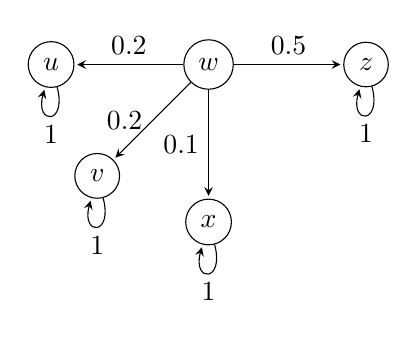
\begin{tikzpicture}[->,>=stealth,shorten >=1pt,auto,node distance=2cm]
        
        % Nodes
        \node[circle,draw] (w) {$w$};
        \node[circle,draw,below left of=w] (v) {$v$};
        \node[circle,draw,left of=w] (u) {$u$};
        \node[circle,draw,below of=w] (x) {$x$};
        \node[circle,draw,right of=w] (z) {$z$};
        
        % Edges
        \path (w) edge node[left] {$0.2$} (v)
              (w) edge node[above] {$0.2$} (u)
              (w) edge node[left] {$0.1$} (x)
              (w) edge node[above] {$0.5$} (z)
              (u) edge [loop below] node {$1$} (v)
              (v) edge [loop below] node {$1$} (v)
              (x) edge [loop below] node {$1$} (x)
              (z) edge [loop below] node {$1$} (z);
        
        \end{tikzpicture}
        \end{minipage}\begin{minipage}{0.48\linewidth}
        \centering
            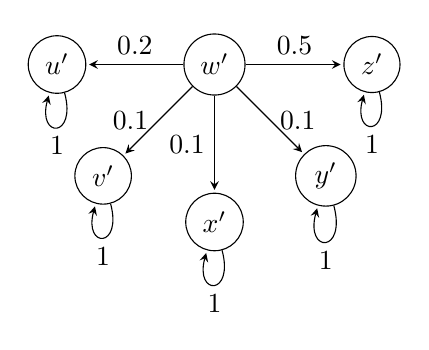
\begin{tikzpicture}[->,>=stealth,shorten >=1pt,auto,node distance=2cm]
        % Nodes
        \node[circle,draw] (w) {$w'$};
        \node[circle,draw, below left of=w] (v) {$v'$};
        \node[circle,draw, left of =w] (u) {$u'$};
        \node[circle,draw,below of=w] (x) {$x'$};
        \node[circle,draw,below right of=w] (y) {$y'$};
        \node[circle,draw,right of=w] (z) {$z'$};
        
        % Edges
        \path (w) edge node[above] {$0.2$} (u)
              (w) edge node[left] {$0.1$} (v)
              (w) edge node[left] {$0.1$} (x)
              (w) edge node[right] {$0.1$} (y)
              (w) edge node[above] {$0.5$} (z)
              (u) edge [loop below] node {$1$} ()
              (v) edge [loop below] node {$1$} (v)
              (x) edge [loop below] node {$1$} (x)
              (y) edge [loop below] node {$1$} (y)
              (z) edge [loop below] node {$1$} (z);
        \end{tikzpicture}
        \end{minipage}
    \caption{Example of models with sabotage bisimilar states.}
    \label{ex_r-bis}
\end{figure}

It is possible to verify that the following relation is a sabotage-bisimulation:
    \[
    \begin{array}{l@{\,}l}
        E = & \{\big((w,P),(w',P')\big),$ $\big((z,P),(z',P')\big)\} \\ 
            & \cup \ \{(t,P)\times (t',P'): \ t\in\{u,v,x\}\text{ and }t'\in\{u',v',x',y'\}\}\\
            & \cup \ \{(z,P^{-(w,z)}_\rho)\times (z',P'^{-(w',z')}_\rho): \ \rho\in ]0,0.5]\}\\
            &\cup \ \{(t,P^{-(w,t)}_\rho)\times (u',P'^{-(w',u')}_\rho): \ t\in\{u,v\}\text{ and }\rho\in]0,0.2]\}\\
            & \cup \ \{(x,P^{-(w,x)}_\rho)\times (t',P'): \ t'\in\{v',x',y'\}\text{ and }\rho\in]0,0.1]\}
    \end{array}
    \]
Therefore, $w$ is bisimilar to $w'$, $z$ is bisimilar to $z'$ and $u$, $v$, $x$ are bisimilar to $u'$, $v'$, $x'$, $y'$. Furthermore, the two models above satisfy the same sabotage formulas by Theorem~\ref{th:invariance}.

\end{example}

\subsection{Hennessy-Milner Results}
\label{sec:henmilner}

In this section, we will devote ourselves to the proof of Hennessy-Milner results~\cite{vanbenthem1977modal}. Concretely, we will show that under certain circumstances, the converse of Theorem~\ref{th:invariance} holds. As it is usual in modal logics, these conditions involve some finiteness constraint, namely image finiteness or finite models. Below we define classes of models satisfying those conditions, called in general \emph{Hennessy-Milner classes} (see, e.g.,~\cite{BlackburnRV01}).


\begin{definition}
    \label{def:image-finite}
A model $\model=(W,P,V)$ is \emph{image finite} if for all $w\in W$, we have that the set $\{v \in W \mid P(w,v)>0\}$ is finite. We say that $\model$ is \emph{finite} if its set of states $W$ is finite.
\end{definition}
%
\begin{remark}\label{rem:well-formed}
   Let $\model=(W,P,V)$ be an image finite probabilistic Kripke model.  Then, for all ${Q}$ that is well-formed from $P$ for sabotage, we have that $\model=(W,{Q},V)$ is also image finite.
\end{remark}

The two types of models will be relevant in our case. Such as it is done for non-probabilistic sabotage in~\cite{ArecesFH15}, image finite suffices to obtain a Hennessy-Milner class. However, this is not the case for bridge, as in infinite model, there exist  infinitely many possible new edges that can be added. In our probabilistic setting, this situation naturally persists.


\begin{theorem}
    [Hennessy-Milner for sabotage]
     Let $\model=(W,P,V)$ and $\model'=(W',P',V')$ be two image finite probabilistic Kripke models. Let ${Q},{Q'}$ be two well-formed probabilistic matrices for sabotage w.r.t. $P,P'$ respectively.  
    Then, $(W,{Q},V),w\equiv_{\mathsf{sb}}(W',{Q}',V'),w'$ implies there exists a sabotage bisimulation $E$ such that $(w,{Q})E(w',{Q}')$.
\end{theorem}
\begin{proof}
We will prove the relation given by:
% \textcolor{blue}{RF: $\bar P$ and ${Q'}$ must all be image finite, to make sure that we always work with image finite models}
\begin{align*}
    E := & \{ ((u,{Q}),(u',{Q}')) \mid  (W,{Q},V), u \equiv_{\mathsf{sb}} (W',{Q}',V') , u' \text{ and } \\
    & \text{ ${Q},{Q'}$ are well-formed for sabotage from $P,P'$ respectively} \} 
\end{align*}
is a sabotage bisimulation. Thus, for every $\big((w,{Q}) ,(w',{Q}')\big)\in E$, we have to prove that conditions \textbf{(atom)}, \textbf{(sab-zig)}, \textbf{(sab-zag)}, and \textbf{(p-zigzag)} hold. Notice that by Remark~\ref{rem:well-formed}, models whose underlying probability matrices are ${Q}$ and ${Q}'$, are image-finite models.
% While doing so, we will denote $\bar{\model}=(W,{Q},V)$ and $\bar{\model}'=(W',{Q}',V)$.

\begin{description}
    \item[(atom):] follows immediately from definition of $E$. 

    \item[\textbf{(sab-zig)}:] let $u \in W$ be such that $\rho \leq {Q}(w,u) \neq 1$. We have to prove that there exists $u'$ such that items 1 and 2 from \textbf{(sab-zig)} hold. First, notice that, since $\rho \neq 1 $, we have that $(W,{Q},V), w \models \blacklozenge_{\rho} \top$. Thus, we also have that $(W',{Q}',V'), w' \models \blacklozenge_{\rho} \top$ (by definition of $E$). Therefore, there exists $u' \in W'$ such that $\rho \leq {Q}'(w',u') \neq 1$, proving item 1. To prove item~2, aiming for a contradiction we assume that for every $u' \in W'$ such that $ \rho \leq {Q}'(w', u') < 1$,  we have $\big(\big(u, {Q}_{\rho}^{-(w,u)}\big), \big(u', {Q}'^{-(w',u')}_{\rho}\big)\big) \notin E$. So, for each such $u'$ there exists $\varphi'$ such that $(W,{Q}^{-(w,u)}_{\rho},V),u\models \varphi'$ and $(W',{Q}'^{-(w',u')}_{\rho},V'),u'\not\models \varphi'$. Since $(W',{Q}'^{-(w',u')}_{\rho},V')$ is image finite, we have only a finite set $\{u'_1,\dots,u'_n\}$ of worlds satisfying the condition. Thus there are $\{ \varphi_1,\dots,\varphi_n \}$ such that $(W,{Q}^{-(w,u)}_{\rho},V),u\models \varphi_i$ and $(W',\bar{P'_{\rho}}^{-(w',u'_i)},V'),u'_i\not\models \varphi_i$. Let us define $\varphi = \bigwedge \varphi_i$, we get a contradiction because $(W,{Q},V), w \models \blacklozenge_{\rho} \varphi$ but $(W',{Q}',V'), w' \not\models \blacklozenge_{\rho} \varphi$. Hence, item 2 holds. Condition \textbf{(sab-zag)} follows in an analogous way.

    \item[\textbf{(p-zigzag)}:] 
    let $U \subseteq W$ and set $\rho = \sum_{u \in U} {Q}(w,u)$. We define the following subsets of $W'$:
    \begin{align*}
          U' &= \{ u' \in W'\mid \text{there exists } u\in U \text{ such that } (u',{Q}')\in E[(u,{Q})] \} \\
          T' &= W' \setminus U' 
    \end{align*}
    Also we define $U_0 = \{u\in U \mid {Q}(w,u) > 0 \}$ and $T'_0 = \{u'\in T' \mid {Q}'(w',u') > 0\}$. Since the models are image finite, $U_0$ and $T'_0$ are finite. Take $u\in U_0$ and $v' \in T'_0$. Since $(v', {Q}') \notin E[(u,{Q})]$, there is $\varphi_{v'}^{u}\in\form $ such that $(W,{Q},V) , u \models \varphi_{v'}^{u}$ and $(W',{Q}',V') , v' \not\models \varphi_{v'}^{u}$. Clearly, the formula
    \[
        \varphi = \bigvee_{u\in U_0} \bigwedge_{v'\in T'_0} \varphi_{v'}^{u}
    \]
    is well-formed, by finiteness of $U_0$ and $T'_0$. 
    By construction, $(W,{Q},V), w \models \Diamond_\rho \varphi$, so $(W',{Q}',V') , w' \models \Diamond_\rho \varphi$ necessarily holds. Thus,
    \[
        \sum_{\{u'\in W' \mid (W',{Q}',V'),u' \models \varphi \}}{Q}(w',u')\geq \rho.
    \]
    Finally, observe that 
    \[ 
        \begin{array}{lcl}            
            W'\setminus T'_0 & =& \{u'\in W' \mid  (u',{Q}')\notin E[(u,{Q})] \text{ or } {Q}'(w',u')=0\} \\
                            & =&  U' \cup (T'\setminus T'_0)
        \end{array}
    \]
    From that observation, we obtain $\{u' \in W' \mid (W',{Q}',V'),u' \models \varphi \} \subseteq W' \setminus T'_0 = U' \cup (T' \setminus T'_0) $, yielding the following inequalities:
    \begin{align*}
        \rho &\leq \sum_{\{u'\in W' \mid (W',{Q}',V'),u' \models \varphi \}}{Q}(w',u') \\
        &\leq \sum_{u'\in U'\cup (T'\setminus T'_0)}{Q}(w',u')\\
        &= \sum_{u'\in U'}{Q}(w',u') + \sum_{T'\setminus T'_0}{Q}(w',u')\\
        &= \sum_{u'\in U'}{Q}(w',u') + 0 \qedhere
    \end{align*}
    %let $U \subseteq W$ and set $\rho = \sum_{u \in U} P(w,u)$. We define the following two subsets of $W'$:
    %    \begin{align*}
      %      U' &= \{ u' \mid \text{there exists } u\in U \text{ such that } (u',P')\in E[(u,P)] \} \\
      %     V' &= W' \setminus U' 
     %   \end{align*}
    %We want to show that $\sum_{u'\in U'} P'(w',u') \geq \rho$. Given $u\in U$ and $v' \in V'$, since $(v', P') \notin E[(u,P)]$, there is $\varphi_{v'}^{u}\in\form $ such that $\model , u \models \varphi_{v'}^{u}$ and $\model' , v' \not\models \varphi_{v'}^{u}$. As the models are image finite, we have that $\varphi = \bigvee_{u\in U} \bigwedge_{v'\in V'} \varphi_{v'}^{u} $ belongs to $\form$.
    %By construction, it follows that $\model , w \models \Diamond_\rho \varphi$, so $\model' , w' \models \Diamond_\rho \varphi$ and since $\varphi$ only holds for $U'$, we have that $\sum_{u'\in U'}P(w',u')\geq \rho $.
\end{description}
\end{proof}

Once a Hennessy-Milner result for sabotage has been established over models with image finite, we proceed to prove a similar result for bridge. Similarly to its non probabilistic counterpart, for bridge the result holds over finite models.

\begin{theorem}
    [Hennessy-Milner for bridge]
     Let $\model=(W,P,V)$ and $\model'=(W',P',V')$ be two finite probabilistic Kripke models.
    Let ${Q},{Q'}$ be two well-formed probabilistic matrices for bridge w.r.t. $P,P'$ resp.  
    Then, $(W,{Q},V),w\equiv_{\mathsf{br}}(W',{Q}',V'),w'$ implies there exists a bridge bisimulation $E$ s.t. $(w,{Q})E(w',{Q}')$.
\end{theorem}
\begin{proof}
% Let us define $E$ like in the sabotage case but using the $\equiv_{\mathsf{br}}$ notion. 
We will prove the relation given by:
\begin{align*}
    E := & \{ ((u,{Q}),(u',{Q}')) \mid  (W,{Q},V), u \equiv_{\mathsf{br}} (W,{Q}',V) , u ' \text{ and} \\
    & \text{ ${Q},{Q'}$ are well-formed for bridge from $P,P'$ respectively} \} 
\end{align*}
is a bridge bisimulation. Again, every well-formed ${Q},{Q'}$ are guaranteed to be finite provided that $\model$ and $\model'$ are finite models.

We need to prove that, for  $\big((w,{Q}) ,(w',{Q}')\big)\in E$, conditions \textbf{(atom)}, \textbf{(br-zig)}, \textbf{(br-zag)}, and \textbf{(p-zigzag)} hold. 

\begin{description}
    \item[(atom):] follows immediately from definition of $E$. 

    % \item[(univ):] \textcolor{blue}{To be completed?}

    \item[\textbf{(br-zig)}:] let $u \in W$ be such that ${Q}(w,u) + \rho \leq 1 $. We have to prove that there exists $u'$ such that items 1 and 2 from \textbf{(br-zig)} hold. As in the case for sabotage, it holds that $(W,{Q},V) , w \models \blacklozenge_{\rho} \top $. Since $(w,{Q})E(w',{Q}')$, we have that $(W',{Q}',V') , w' \models \blacklozenge_{\rho} \top $, so there exists $u'$ such that ${Q}'(w',u') + \rho \leq 1$. Thus, item 1 holds. Now, aiming for a contradiction, let us assume item 2 does not hold, i.e., for every $u'\in W'$ such that ${Q}'(w',u') + \rho \leq 1$, we have that $\big ( \big ( u, {Q}_{\rho}^{+(w,u)} \big ), \big ( u',{Q}'^{+(w',u')}_{\rho}\big )\big ) \notin E$. Therefore, for each $u'$ such that ${Q}'(w',u') + \rho \leq 1 $, there exists $\varphi_{u'}$ that satisfies that $(W,{Q},V) , u \models \varphi_u'$ and $(W',{Q}',V') , u' \not \models \varphi_u'$. Since $W'$ is finite, we can define $\varphi = \blacklozenge_\rho \bigwedge \varphi_{u'}$. This yields a contradiction, since $(W,{Q},V) , w \models \varphi$ and $(W',{Q}',V') , w' \not \models \varphi$, hence proving item 2. Condition \textbf{(br-zag)} follows in an analogous way.
    %     \begin{align*}
    %         {Q}'(w',u') + \rho &< 1 \\
    %         {Q}'(w',u') + 1 - {Q}(w,u) - \delta &< 1 \\
    %         {Q}'(w',u') &< {Q}(w,u) + \delta  
    %     \end{align*}
    % Since it holds for every $\delta > 0$, we can take the limit as $\delta$ approaches zero, and we get ${Q}'(w',u') \leq  {Q}(w,u)$. 
    
    \item[\textbf{(p-zigzag)}:] For $U \subseteq W$, let $\rho = \sum_{u \in U} {Q}(w,u)$. Define the following sets:
        \begin{align*}
            U' &= \{ u' \in W' \mid \text{there exists } u\in U \text{ such that } (u',{Q}')\in E[(u,{Q})] \} \\
            T' &= W' \setminus U' 
        \end{align*}
    We need to show that $\sum_{u'\in U'} {Q}'(w',u') \geq \rho$. Given $u\in U$ and $v'~\in~T'$, since $(v', {Q}') \notin E[(u,{Q})]$, there is $\varphi_{v'}^{u}\in\form $ such that $(W,{Q},V) , u \models \varphi_{v'}^{u}$ and $(W',{Q}',V') , v' \not\models \varphi_{v'}^{u}$. As the models are finite, we have that $\varphi = \bigvee_{u\in U} \bigwedge_{v'\in V'} \varphi_{v'}^{u} $ belongs to $\form$.
    By construction, $(W,{Q},V) , w \models \Diamond_\rho \varphi$, so $(W'{Q}',V') , w' \models \Diamond_\rho \varphi$. Since $\varphi$ only holds for $U'$, we have that
    \[
        \sum_{u'\in U'}{Q}(w',u')\geq \rho. \qedhere
    \]
\end{description}
\end{proof}


We finish this section with the corresponding Hennessy-Milner result under swap semantics. 

\begin{theorem}
    [Hennessy-Milner for swap]
    Let $\model=(W,P,V)$ and $\model'=(W',P',V')$ be two image finite probabilistic Kripke models. Let ${Q},{Q'}$ be two well-formed probabilistic matrices for swap w.r.t. $P,P'$ respectively.  
    Then, $(W,{Q},V),w\equiv_{\mathsf{sw}}(W',{Q}',V'),w'$ implies there exists a swap bisimulation $E$ such that $(w,{Q})E(w',{Q}')$.
\end{theorem}
\begin{proof}
We will prove the relation given by:
\begin{align*}
    E := & \{ ((u,{Q}),(u',{Q}')) \mid  (W,{Q},V), u \equiv_{\mathsf{sw}} (W,{Q}',V) , u ' \text{ and} \\
    & \text{ ${Q},{Q'}$ are well-formed for swap from $P,P'$ respectively} \} 
\end{align*}
is a swap bisimulation. % Again, every well-formed ${Q},{Q'}$ are guaranteed to be finite provided that $\model$ and $\model'$ are finite models.

We need to prove that, for  $\big((w,{Q}) ,(w',{Q}')\big)\in E$, conditions \textbf{(atom)}, \textbf{(sw-zig)}, \textbf{(sw-zag)}, and \textbf{(p-zigzag)} hold. 

\begin{description}
    \item[(atom):] follows immediately from definition of $E$. 

    \item[(sw-zig):] let $u \in W$ be such that $\rho \leq Q(w,u) \neq 1 $ and $Q(u,w) + \rho \leq 1$. We have to prove that there exist $u'$ such that items 1 and 2 from \textbf{(sw-zig)} hold. We can say that $(W,{Q},V) , w \models \blacklozenge_{\rho} \top $. Since $\big((w,{Q}) ,(w',{Q}')\big)\in E$, we have that $(W',{Q}',V') , w' \models \blacklozenge_{\rho} \top $, so there exists $u'$ such that $\rho \leq Q(w',u') \neq 1 $ and $Q(u',w') + \rho \leq 1$, proving item 1. To prove item 2, we assume that for every $u' \in W'$, such that $\rho \leq Q(w',u') \neq 1$ and $Q(u',w') + \rho \leq 1$, we have $\big ( \big ( u, {Q}_{\rho}^{*(w,u)} \big ), \big ( u',{Q}'^{*(w',u')}_{\rho}\big )\big ) \notin E$. So, for each $u'$ there exists $\varphi'$ such that $(W,{Q}^{*(w,u)}_{\rho},V) , u \models \varphi'$ and $(W',{Q}'^{*(w',u')}_{\rho},V') , u' \not \models \varphi'$.

\end{description}

\end{proof}
\section{Case Study}
\label{sec:case}

We conclude by presenting a concrete application of our probabilistic relation-changing framework. Specifically, we illustrate how our logics can be employed to reason about a biological scenario, drawing inspiration from~\cite{ATHGM16}. 

Cells are often subjected to stress for various reasons, including viral infections, replication errors, and exposure to harmful chemicals. In response, cells attempt to repair the resulting damage and maintain their normal functioning. However, when repair is unsuccessful, cells may trigger apoptosis (programmed cell death).

In this paper, we consider a simplified model of cellular dynamics in which DNA damage is caused by ionizing radiation, such as that associated with X-ray imaging procedures, leading to the occurrence of double-strand breaks (DSBs). In~\cite{ATHGM16}, the authors provide evidence that, even after the initial damage has been repaired, the accumulation of residual DSBs increases the likelihood of subsequent repair failure and, consequently, of apoptosis. Inspired by this case study, we propose a deliberately simplified, illustrative transition model (called hereafter $\model$) of these cellular dynamics, depicted in Fig.~\ref{ex_apop}. We emphasize that this is not intended to be a biologically rigorous model: the probabilities assigned to the transitions are purely illustrative.

\begin{figure}
\centering
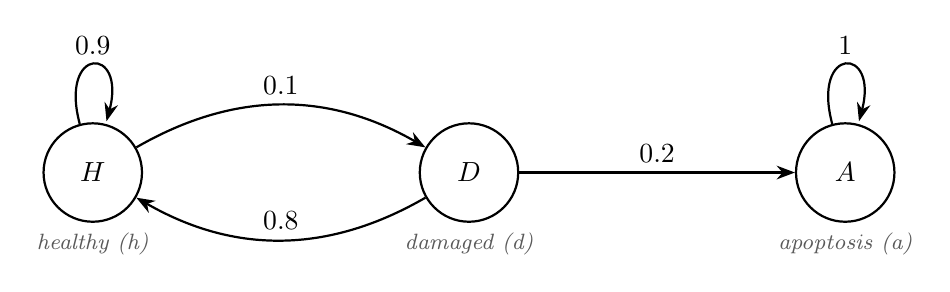
\begin{tikzpicture}[
    >=Stealth,
    node distance=3.5cm,
    every state/.style={thick, minimum size=1.25cm},
    every edge/.style={draw, ->, thick},
    prob/.style={font=\small, fill=white, inner sep=1.4pt},
    prop/.style={font=\footnotesize\itshape, text=gray!70!black}
]
 
\node[state, label={[prop]below:healthy (h)}]   (H) {$H$};
\node[state, right=of H, label={[prop]below:damaged (d)}]  (D) {$D$};
\node[state, right=of D, label={[prop]below:apoptosis (a)}] (A) {$A$};
 
% Transitions 

\path
  (H) edge[loop above]  node[above] {0.9} (H)
      edge[bend left]  node[above] {0.1} (D)
  (D) edge[bend left]  node[above] {0.8} (H)
      edge [] node[above] {0.2} (A)
  (A) edge[loop above] node[above] {1}   (A);
 
\end{tikzpicture}
\caption{A conceptual model for cell apoptosis after DSB lesion on its DNA.}
\label{ex_apop}
\end{figure}

The model $\M=(W,P,V)$ consists of three states, namely, $W=\{h,d,a\}$, representing the cell being $healthy$ ($h$), $damaged$ ($d$), or undergoing $apoptosis$~($a$). The transition probabilities are given by the matrix shown in Table~\ref{ex_matrix}. The valuation function $V:\{H,D,A\}\rightarrow 2^W$ assigns the following sets of states to the respective atomic propositions: $V(H)=\{h\}$, $V(D)=\{d\}$, and $V(A)=\{a\}$.


\begin{table}[h!]
    \centering
        \caption{Transition probability matrix of model depicted in Fig. \ref{ex_apop}.}
    \begin{tabular}{|c|c c c|}
        \hline
         $\hspace{2.5cm}$&$healthy \ (h)$&$damaged \ (d)$&$apoptosis \ (a)$ \\\hline
         $healthy \ (h)$&0.9&0.1&$\hspace{2.5cm}$\\
         $damaged \ (d)$&0.8&&0.2\\
         $apoptosis \ (a)$&$\hspace{2.5cm}$&$\hspace{2.5cm}$& 1\\ \hline
    \end{tabular}
    \label{ex_matrix}
\end{table}


While such a simple model is easy to understand, it fails to fully capture the complex dynamics of the system. Indeed, the fact that cumulative DSB lesions lead to an increased risk of cellular apoptosis, is not captured by it. Nevertheless, relation-changing operators can be used to naturally describe changes in transition probabilities.

For instance, consider the formula $\Diamond_{0.3} A$, that holds whenever:

\medskip

\textit{The probability of transitioning to an $apoptosis$ state in the next step is at least $0.3$.}

\medskip

Thus, one can check that $\M,d\not\models\Diamond_{0.3} A$, because the probability of going from state $damaged$ to $apoptosis$ is only $0.2$ and $A$ holds at no other state.

% However, consider the following formula, with $\blacklozenge$ being the probabilistic sabotage operator: 
However, if we assume that after the cell repairs from a lesion, the probability of the cell to repair again and return to the healthy state reduces by $0.1$, we may consider the following formula, with $\blacklozenge$ being the probabilistic sabotage operator:
\[ 
    \blacklozenge_{0.1} \big(H \wedge \Diamond_1 (H \vee \Diamond_{0.3} A )\big).
\]
When evaluated at the state $damaged$, this formula expresses that:

\medskip

% \textit{If whenever a cell repairs from a DSB lesion, it reduces the probability of the cell to repair again and return to the $healthy$ state by 0.1 after a new lesion occurs, then when a new lesion occurs, the probability of apoptosis to be induced is now greater or equal than 0.3.}
% \textit{After repairing from a lesion, a cell may either remain healthy or suffer a new lesion that triggers apoptosis with a probability of at least $0.3$.}

\textit{There is an admissible repair update leading to a healthy state from which, with probability one, a cell may either remain healthy or suffer a new lesion that triggers apoptosis with a probability of at least $0.3$.}

\medskip

Let us proceed to evaluate the formula at state $d$. To do so, let us define:
\[
    \M'=(W,P',V), \qquad \text{ with } P'=P^{-(d,h)}_{0.1}.
\]
Since $H$ holds only at $h$ and $P(d,h)=0.8$, the only possible witness for
the sabotage operator is $h$. The update transfers probability from the
transition $(d,h)$ to the other outgoing transition, so
\[
    P'(d,a)
    =P(d,a)+\frac{0.1\cdot P(d,a)}{1-P(d,h)}
    =0.2+\frac{0.1\cdot0.2}{1-0.8}
    =0.3.
\]
Thus $\M',d\models\Diamond_{0.3}A$. Also,
$\M',a\models\Diamond_{0.3}A$ since $P'(a,a)=1$, and
$\M',h\models H$. Consequently, every state satisfies
$H\vee\Diamond_{0.3}A$. The outgoing probabilities from $h$ are unchanged,
with $P'(h,h)=0.9$, $P'(h,d)=0.1$, and $P'(h,a)=0$. Therefore,
\begin{align*}
   &  \M,d\models\blacklozenge_{0.1}
        \bigl(H\wedge\Diamond_1(H\vee\Diamond_{0.3}A)\bigr)\\
    \iff \quad  & \M',h\models
        H\wedge\Diamond_1(H\vee\Diamond_{0.3}A)\\
    \iff \quad  & \sum_{\substack{x\in W\\
        \M',x\models H\vee\Diamond_{0.3}A}}P'(h,x)\geq 1\\
    \iff \quad & P'(h,h)+P'(h,d)+P'(h,a)\geq 1\\
    \iff \quad & 0.9+0.1+0\geq 1, %\\
    % \iff \quad & \text{true}.
\end{align*}
which is true. The reasoning above illustrates how the use of the probabilistic sabotage operator is useful in such contexts to describe reconfigurable scenarios or where some kind of memory can affect the probability of an edge.

In a similar way, we could use the bridge for modeling scenarios such as cases of immune cells that increase their efficacy while responding to repeated infections by the same virus.
\section{Conclusion and future work}\label{sec:final}

In this paper, we extend the paradigm of relation-changing logics to probabilistic relational structures. While traditional relation-changing logics address dynamic phenomena over discrete models, we adapt this framework to settings where transitions are governed by probabilities. Specifically, we introduce three novel relation-changing operators tailored to the probabilistic case and analyze their impact on the underlying semantics, namely, local sabotage, bridge, and swap modalities. These operators are inspired by~\cite{ArecesFH15} and are designed to represent transition deletion, addition, and reversal, respectively. To support reasoning in this setting, we also investigate appropriate notions of probabilistic bisimulation, showing how these operators interact with key behavioral equivalences. This work thus opens a new direction in the study of relation-changing logics, complementing existing proposals in paraconsistent, fuzzy, and graded contexts~\cite{CostaFM23,FFM25}.

This work is closely related to graded relation updates from~\cite{FFM25}, where classical relation-changing operators are extended to graded (fuzzy) relational structures. While that approach captures degree-based updates of accessibility, our proposal focuses on distributional updates over probabilistic transition systems, thus providing a complementary perspective on extending relation-changing logics beyond the classical setting. Moreover, unlike the approach in~\cite{FFM25}, we focus on a \emph{crisp} semantics, i.e., the truth value of a formula is ultimately true or false, whereas in the aforementioned work, formulas are interpreted with different degrees of truth.

We introduced the syntax, semantics, and examples for the three kinds of updates, and then studied the associated notions of bisimulation. We prove that these notions properly capture structural properties of the respective logics. Concretely, we establish invariance theorems and characterize appropriate Hennessy-Milner classes of models. We also present a case study to illustrate how our framework can be used for reasoning in real-life scenarios.  
Our developments can be considered a starting point for this perspective on probabilistic updates and their applications.

As future work, we aim to develop model-checking tools for probabilistic relation-changing logics. Although developed in a different context, rPRISM~\cite{FRMC19} -- a tool integrated with PRISM -- could serve as a starting point. We also plan to investigate the decidability status and complexity of the model-checking problem and develop an automatic model checker that integrates probabilistic sabotage, bridge, and swap operators. Furthermore, other reasoning tasks for probabilistic relation-changing logics remain unexplored. In particular, defining axiomatic systems, especially tableau-based methods inspired by, e.g.,~\cite{ArecesFH13,Fervari14,KozhemiachenkoS26}, and developing corresponding implementations extending, e.g.,~\cite{HoffmannA09,ArecesFHM16}, are promising directions for further research.

Another direction concerns the exploration of alternative semantics for rel\-ation-changing operators. In our approach, the operators are defined so that, after the model is changed, we move to a new accessible state (with an appropriate probability). An alternative would be to update the model without moving from the current state (see, e.g.,~\cite{GierasimczukKV09}). We also plan to investigate global versions of these operators, in which changes are not made locally but can occur anywhere in the transition probability matrix of the model. A further possibility is to define general probabilistic updates, as done in~\cite{ArecesFH15} for the non-probabilistic cases. Finally, restricted variants of the operators, designed for particular purposes as in epistemic logic, deserve further attention, particularly regarding their logical consequences for decidability and expressivity.

% Finally, we intend to explore the existence of a Hennessy-Milner theorem for finite models concerning our definition of bisimulation in the probabilistic setting, as well as in the model changing case.



\paragraph{Acknowledgments}
D. Figueiredo and M. A. Martins acknowledge the support of CIDMA (\url{https://ror.org/05pm2mw36})
under the Portuguese Foundation for Science and Technology 
(FCT, \url{https://ror.org/00snfqn58}), Grants UID/\allowbreak 04106/\allowbreak 2025 (\href{https://doi.org/10.54499/UID/04106/2025}{DOI}) 
and UID/\allowbreak PRR/\allowbreak 04106/\allowbreak 2025; and European Funds through SACCCT- IC\&DT - Sistema de Apoio \`a Cria\c c\~ao de Conhecimento Cient\'ifico e Tecnol\'ogico, as part of COMPETE2030, within the project BANKSY with reference number 15253.
R. Fervari is supported by 
%
the EU H2020 research and innovation programme
under the Marie Sk{\l}odowska-Curie grant agreements 101008233
({MISSION}),
%
the IRP SINFIN, 
%
and SeCyT-UNC grant 33620230100178CB.

\bibliographystyle{plain}
\bibliography{ref}

\end{document}